
\documentclass{article}

\usepackage{fancyhdr} % Required for custom headers
\usepackage{lastpage} % Required to determine the last page for the footer
\usepackage{extramarks} % Required for headers and footers
\usepackage[usenames,dvipsnames]{color} % Required for custom colors
\usepackage{graphicx} % Required to insert images
\usepackage{listings} % Required for insertion of code
\usepackage{courier} % Required for the courier font
\usepackage{lipsum} % Used for inserting dummy 'Lorem ipsum' text into the template
\usepackage{caption}
\usepackage{subcaption}
\usepackage{amsmath}
\usepackage[utf8]{inputenc}

\graphicspath{ {figures} }

% Margins
\topmargin=-0.45in
\evensidemargin=0in
\oddsidemargin=0in
\textwidth=6.5in
\textheight=9.0in
\headsep=0.25in

\linespread{1.1} % Line spacing

% Set up the header and footer
\pagestyle{fancy}
\lhead{\hmwkAuthorName} % Top left header
\chead{\hmwkClass\ (\hmwkClassInstructor\ \hmwkClassTime): \hmwkTitle} % Top center head
\rhead{\firstxmark} % Top right header
\lfoot{\lastxmark} % Bottom left footer
\cfoot{} % Bottom center footer
\rfoot{Page\ \thepage\ of\ \protect\pageref{LastPage}} % Bottom right footer
\renewcommand\headrulewidth{0.4pt} % Size of the header rule
\renewcommand\footrulewidth{0.4pt} % Size of the footer rule

\setlength\parindent{0pt} % Removes all indentation from paragraphs

%----------------------------------------------------------------------------------------
%	CODE INCLUSION CONFIGURATION
%----------------------------------------------------------------------------------------

\definecolor{MyDarkGreen}{rgb}{0.0,0.4,0.0} 
\lstloadlanguages{Matlab}
\lstset{language=Matlab,
        frame=single,
        basicstyle=\small\ttfamily,
        keywordstyle=[1]\color{Blue}\bf,
        keywordstyle=[2]\color{Purple},
        keywordstyle=[3]\color{Blue}\underbar,
        identifierstyle=,
        commentstyle=\usefont{T1}{pcr}{m}{sl}\color{MyDarkGreen}\small, 
        stringstyle=\color{Purple},
        showstringspaces=false,
        tabsize=5, 
        morekeywords={rand},
        morekeywords=[2]{on, off, interp},
        morekeywords=[3]{test},
        morecomment=[l][\color{Blue}]{...},
        numbers=left,
        firstnumber=1,
        numberstyle=\tiny\color{Blue},
        stepnumber=5
}

% Creates a new command to include a perl script, the first parameter is the filename of the script (without .pl), the second parameter is the caption
\newcommand{\matlabscript}[2]{
\begin{itemize}
\item[]\lstinputlisting[caption=#2,label=#1]{#1.m}
\end{itemize}
}

%----------------------------------------------------------------------------------------
%	DOCUMENT STRUCTURE COMMANDS
%	Skip this unless you know what you're doing
%----------------------------------------------------------------------------------------

% Header and footer for when a page split occurs within a problem environment
\newcommand{\enterProblemHeader}[1]{
\nobreak\extramarks{#1}{#1 continued on next page\ldots}\nobreak
\nobreak\extramarks{#1 (continued)}{#1 continued on next page\ldots}\nobreak
}

% Header and footer for when a page split occurs between problem environments
\newcommand{\exitProblemHeader}[1]{
\nobreak\extramarks{#1 (continued)}{#1 continued on next page\ldots}\nobreak
\nobreak\extramarks{#1}{}\nobreak
}

\setcounter{secnumdepth}{0} % Removes default section numbers
\newcounter{homeworkProblemCounter} % Creates a counter to keep track of the number of problems

\newcommand{\homeworkProblemName}{}
\newenvironment{homeworkProblem}[1][Problem \arabic{homeworkProblemCounter}]{ % Makes a new environment called homeworkProblem which takes 1 argument (custom name) but the default is "Problem #"
\stepcounter{homeworkProblemCounter} % Increase counter for number of problems
\renewcommand{\homeworkProblemName}{#1} % Assign \homeworkProblemName the name of the problem
\section{\homeworkProblemName} % Make a section in the document with the custom problem count
\enterProblemHeader{\homeworkProblemName} % Header and footer within the environment
}{
\exitProblemHeader{\homeworkProblemName} % Header and footer after the environment
}

\newcommand{\problemAnswer}[1]{ % Defines the problem answer command with the content as the only argument
\noindent\framebox[\columnwidth][c]{\begin{minipage}{0.98\columnwidth}#1\end{minipage}} % Makes the box around the problem answer and puts the content inside
}

\newcommand{\homeworkSectionName}{}
\newenvironment{homeworkSection}[1]{ % New environment for sections within homework problems, takes 1 argument - the name of the section
\renewcommand{\homeworkSectionName}{#1} % Assign \homeworkSectionName to the name of the section from the environment argument
\subsection{\homeworkSectionName} % Make a subsection with the custom name of the subsection
\enterProblemHeader{\homeworkProblemName\ [\homeworkSectionName]} % Header and footer within the environment
}{
\enterProblemHeader{\homeworkProblemName} % Header and footer after the environment
}

%----------------------------------------------------------------------------------------
%	NAME AND CLASS SECTION
%----------------------------------------------------------------------------------------

\newcommand{\hmwkTitle}{Assignment\ \#2}
\newcommand{\hmwkDueDate}{Monday,\ September\ 11,\ 2017}
\newcommand{\hmwkClass}{Pattern Recognition} % Course/class
\newcommand{\hmwkClassTime}{09:10am} % Class/lecture time
\newcommand{\hmwkClassInstructor}{shkim} % Teacher/lecturer
\newcommand{\hmwkAuthorName}{Tien Anh Nguyen} % Your name

%----------------------------------------------------------------------------------------
%	TITLE PAGE
%----------------------------------------------------------------------------------------

\title{
\vspace{2in}
\textmd{\textbf{\hmwkClass:\ \hmwkTitle}}\\
\normalsize\vspace{0.1in}\small{Due\ on\ \hmwkDueDate}\\
\vspace{0.1in}\large{\textit{\hmwkClassInstructor\ \hmwkClassTime}}
\vspace{3in}
}

\author{\textbf{\hmwkAuthorName}}
\date{} % Insert date here if you want it to appear below your name

%----------------------------------------------------------------------------------------

\begin{document}

\maketitle

%----------------------------------------------------------------------------------------
%	TABLE OF CONTENTS
%----------------------------------------------------------------------------------------

%\setcounter{tocdepth}{1} % Uncomment this line if you don't want subsections listed in the ToC

\newpage
\tableofcontents
\newpage

%----------------------------------------------------------------------------------------
%	PROBLEM 1
%----------------------------------------------------------------------------------------

% To have just one problem per page, simply put a \clearpage after each problem

\begin{homeworkProblem}
\maketitle
\subsection{Exercise 2.4.1}
\matlabscript{mfiles/exercise_02_04_01}{Source codes}

\newpage
\newpage
\begin{figure}[h]
        \centering
        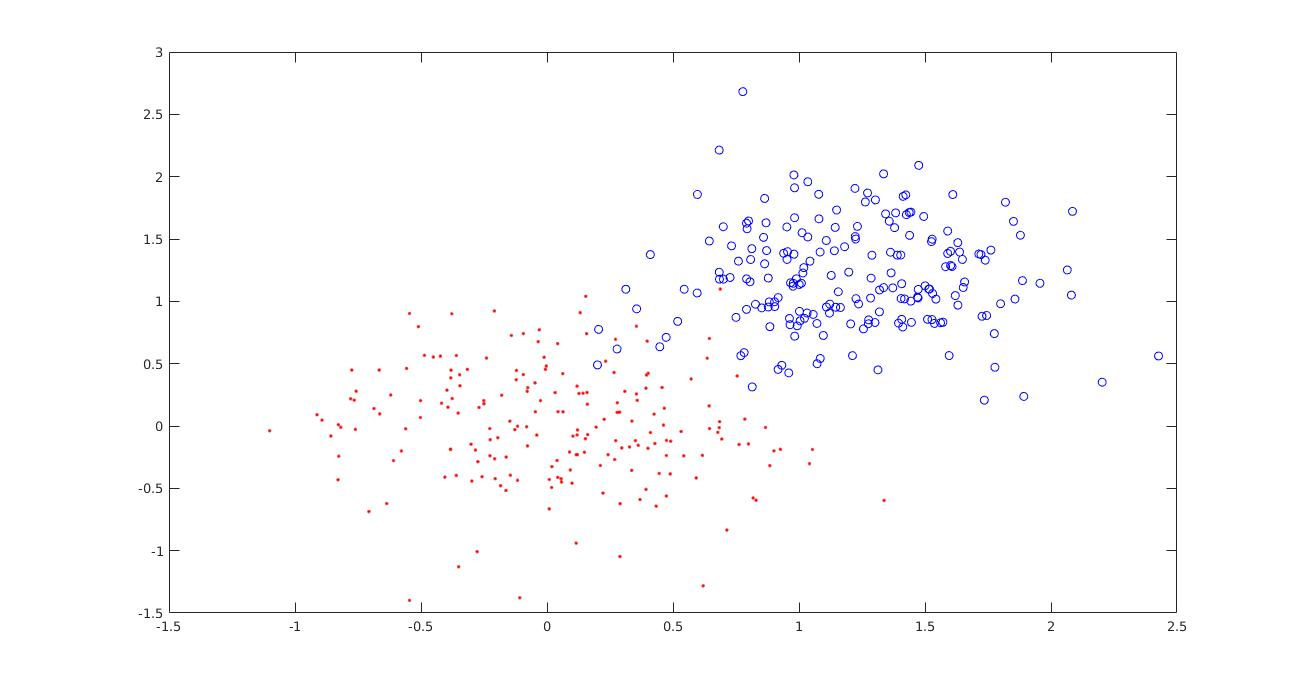
\includegraphics[scale=0.4]{figures/exercise_02_04_01_fig_01.jpg}
        \caption{Training Data X1}
\end{figure}

\newpage

\begin{figure}[h]
\centering
    \begin{subfigure}[h]{0.5\textwidth}
        \centering
        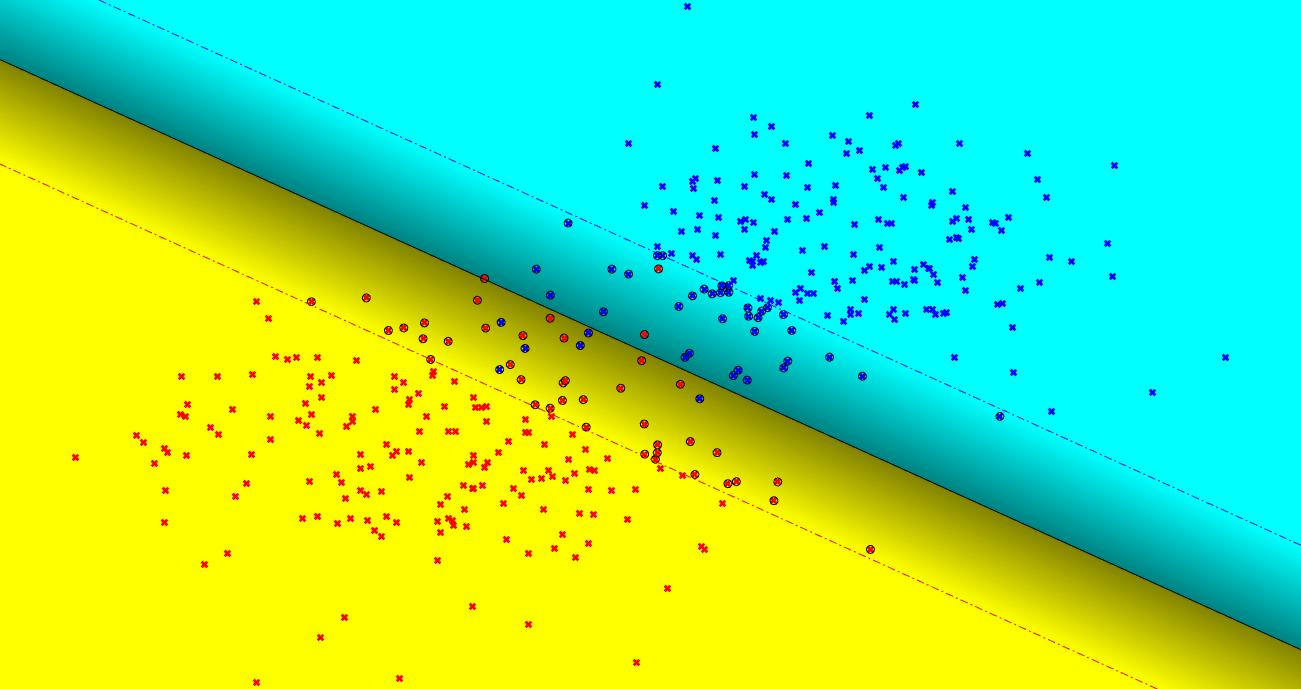
\includegraphics[width=4in,height=3in]{figures/exercise_02_04_01_fig_02.jpg}
        \caption{C=0.1}
    \end{subfigure}\\
    \begin{subfigure}[h]{0.5\textwidth}
        \centering
        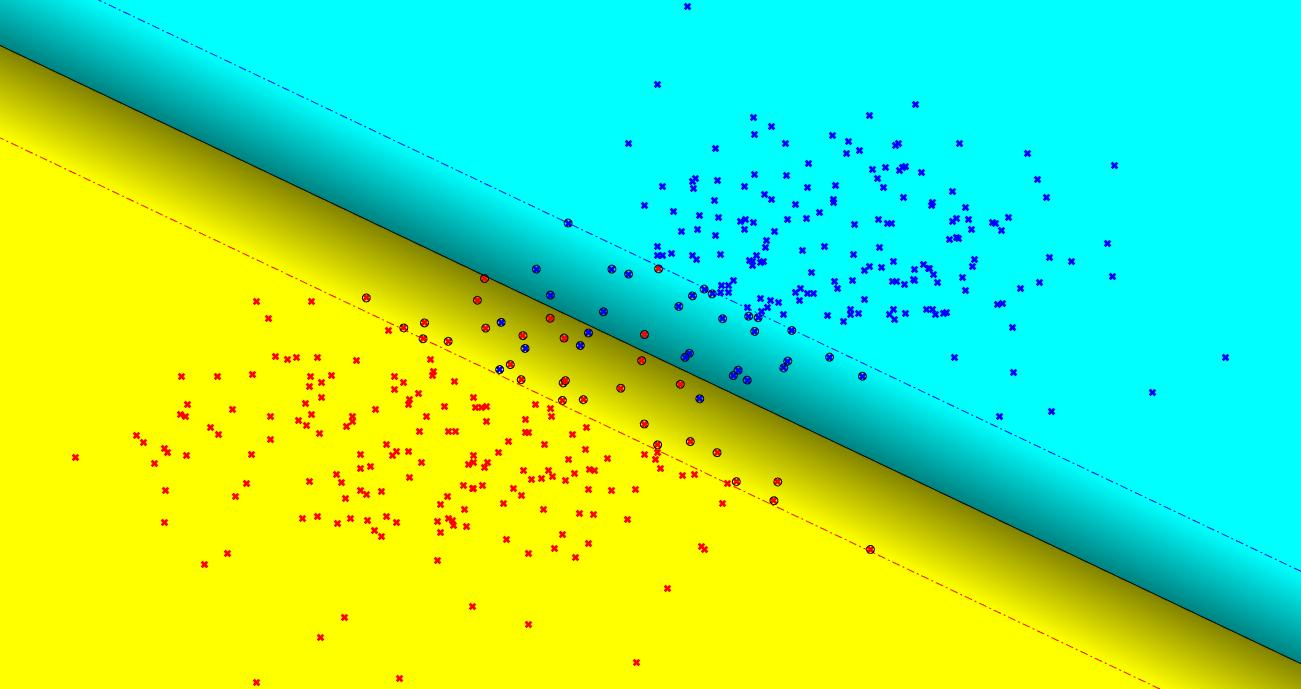
\includegraphics[width=4in,height=3in]{figures/exercise_02_04_01_fig_03.jpg}
        \caption{C=0.2}
    \end{subfigure}
\end{figure}

\newpage

\begin{figure}[h]
\centering
    \begin{subfigure}[h]{0.5\textwidth}
        \centering
        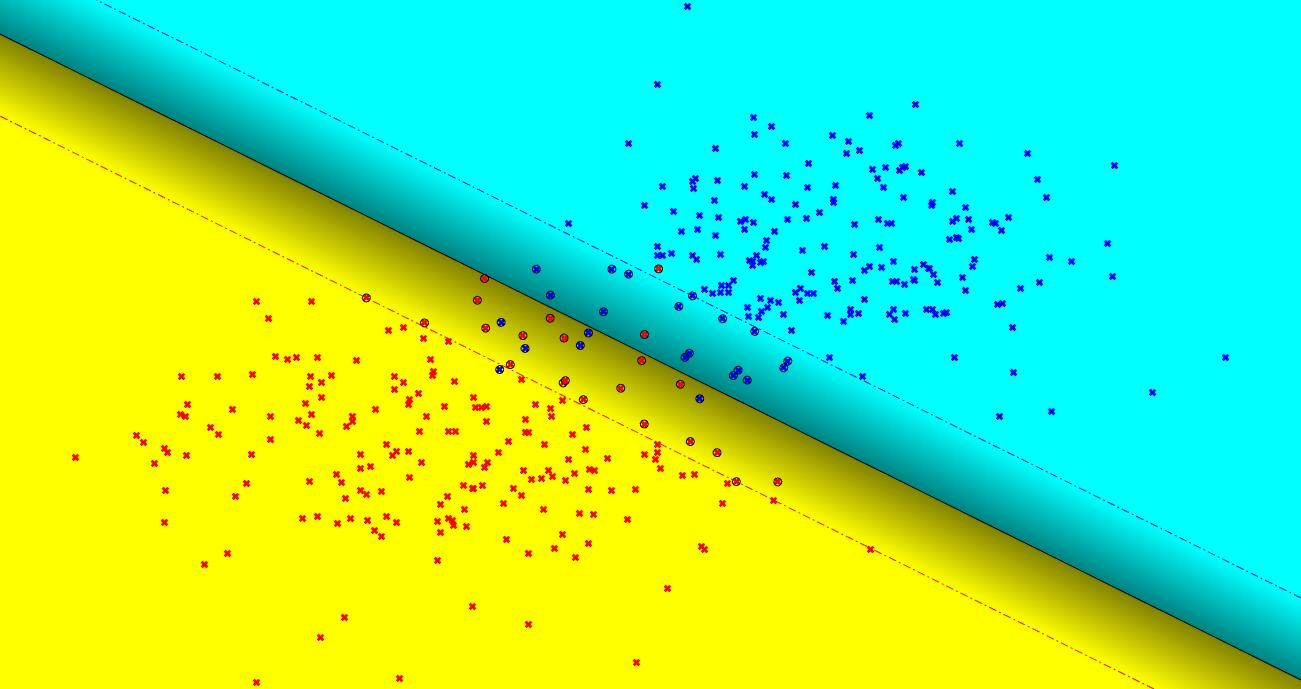
\includegraphics[width=4in,height=3in]{figures/exercise_02_04_01_fig_04.jpg}
        \caption{C=0.5}
    \end{subfigure}\\
    \begin{subfigure}[h]{0.5\textwidth}
        \centering
        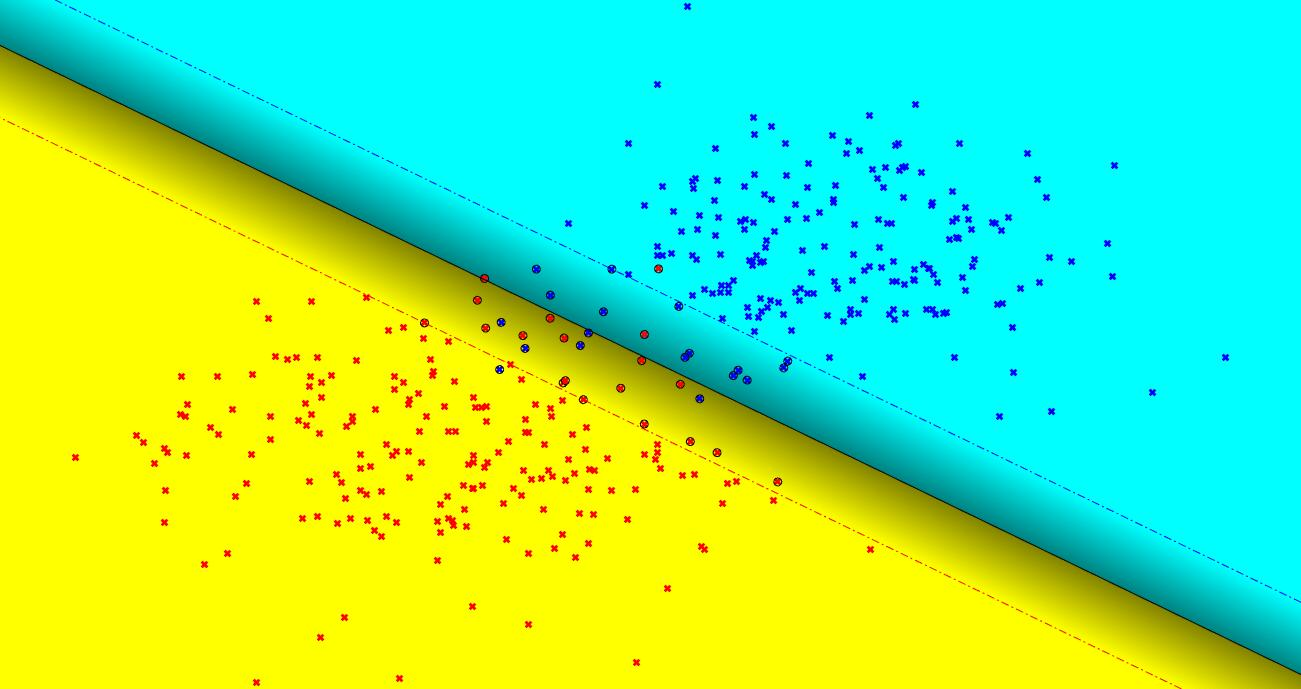
\includegraphics[width=4in,height=3in]{figures/exercise_02_04_01_fig_05.jpg}
        \caption{C=1}
    \end{subfigure}\\
\end{figure}

\newpage

\begin{figure}[h]
\centering
    \begin{subfigure}[h]{0.5\textwidth}
        \centering
        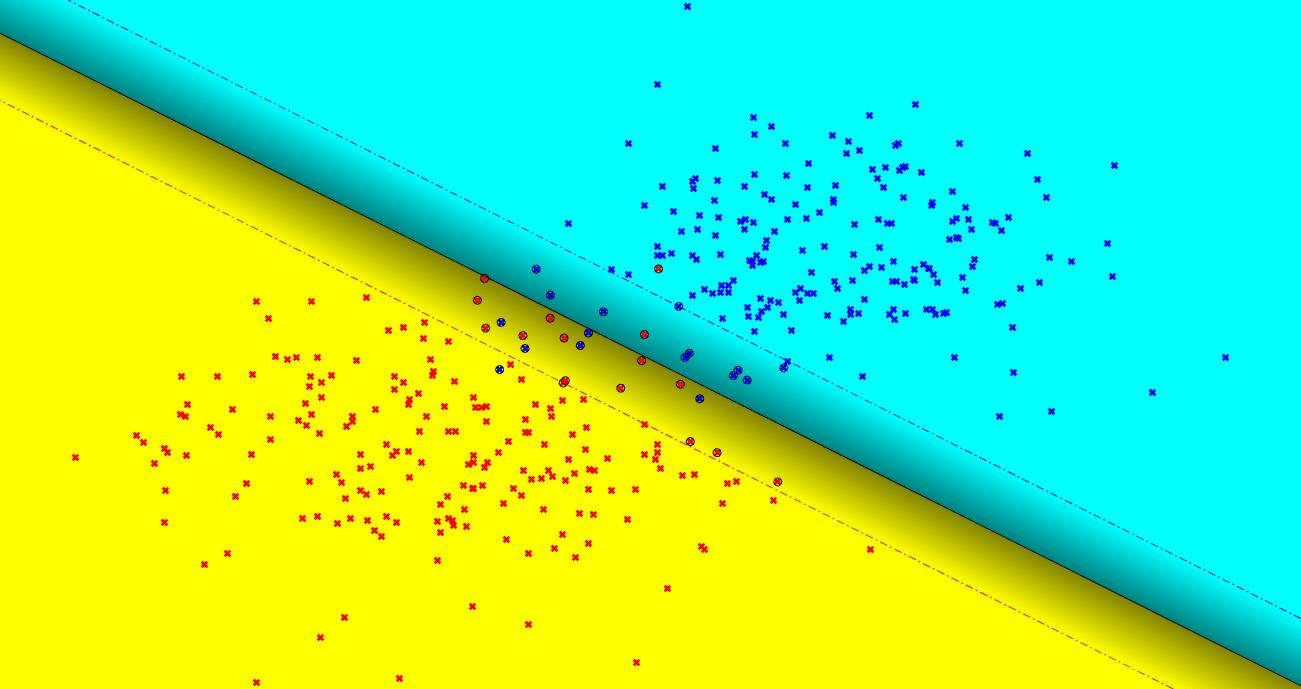
\includegraphics[width=4in,height=3in]{figures/exercise_02_04_01_fig_06.jpg}
        \caption{C=2}
    \end{subfigure}\\
\end{figure}
\begin{figure}[h]
\centering
    \begin{subfigure}[h]{0.5\textwidth}
        \centering
        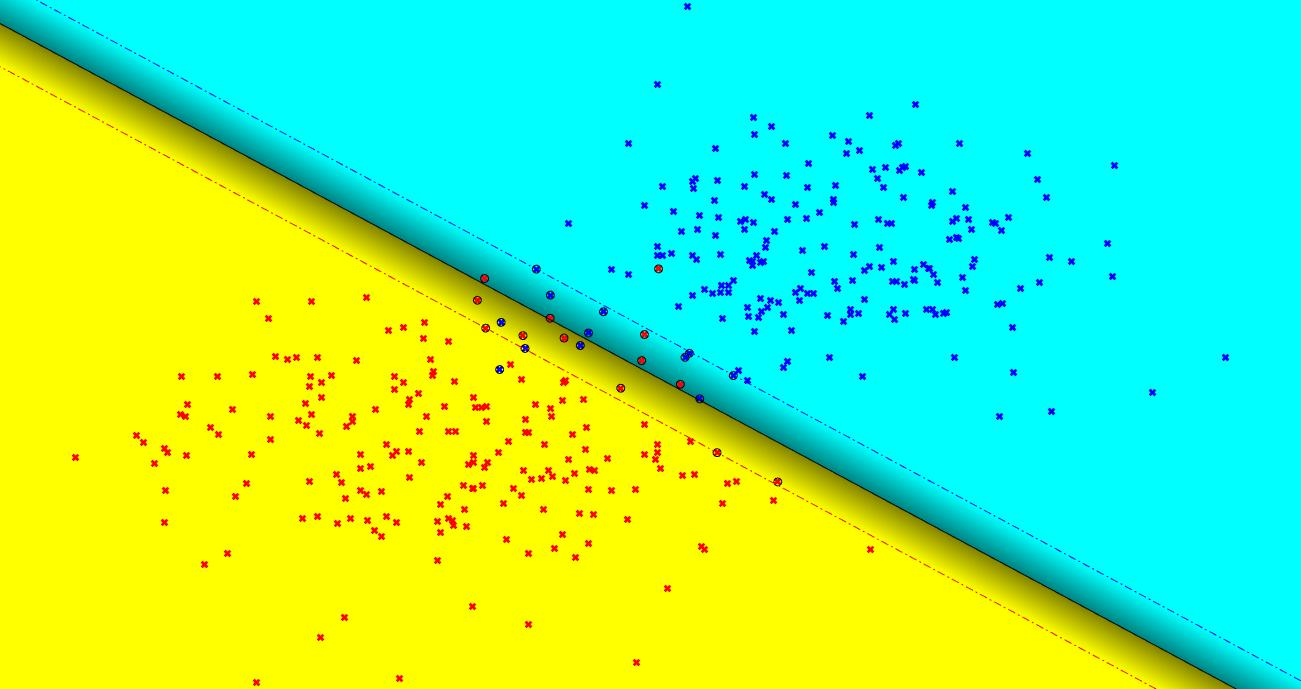
\includegraphics[width=4in,height=3in]{figures/exercise_02_04_01_fig_07.jpg}
        \caption{C=20}
    \end{subfigure}%
\end{figure}

\newpage
\begin{figure}[h]
    \centering
    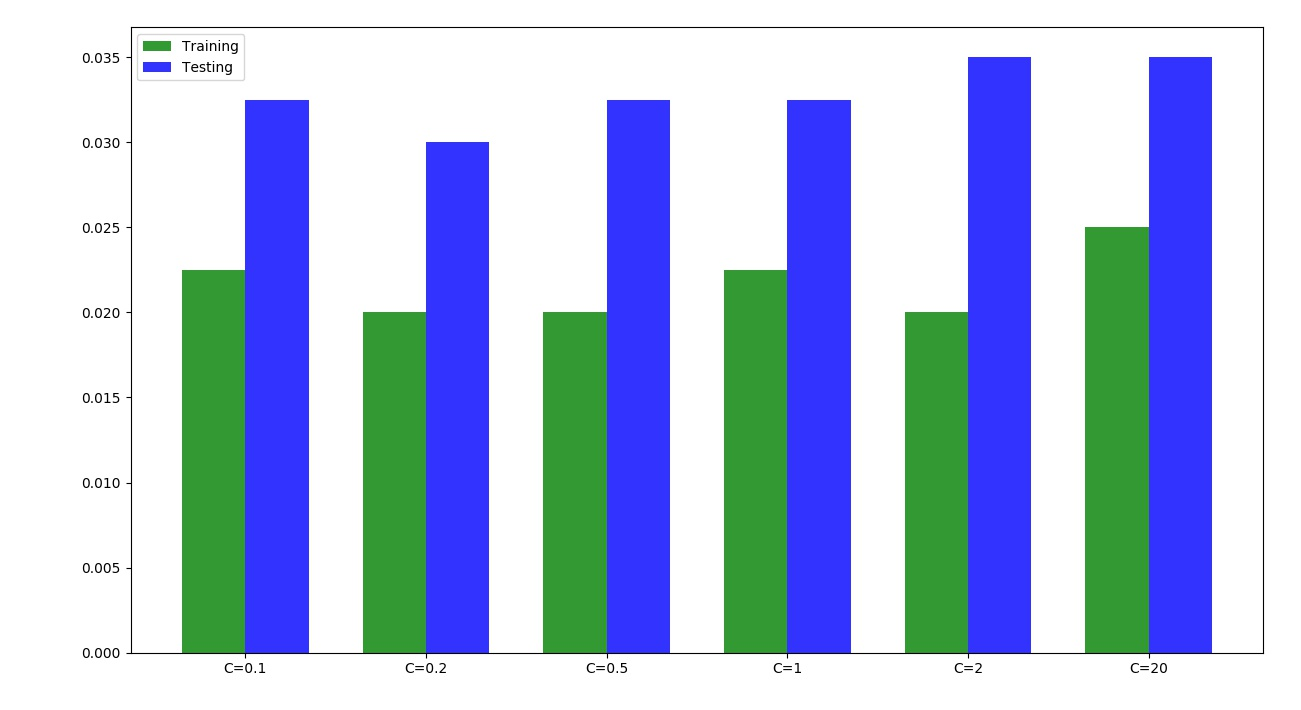
\includegraphics[width=4in,height=3in]{figures/exercise_02_04_01_fig_08.jpg}
    \caption{Testing and Training Errors}
\end{figure}

\begin{center}
\begin{tabular}{ |p{3.5cm}|p{1cm}|p{1cm}|p{1cm}|p{1cm}|p{1cm}|p{1cm}| }
\hline
\multicolumn{7}{|c|}{Testing and Training Errors} \\
\hline
               & C=0.1 & C=0.2 & C=0.5 & C=1 & C=2 & C=20 \\
\hline
Training error & 0.0225 & 0.0200 & 0.0200 & 0.0225 & 0.0200 & 0.0250 \\
Testing error & 0.0325 & 0.0300 & 0.0325 & 0.0325 & 0.0350 & 0.0350 \\
Margin & 0.9414 & 0.8147 & 0.7085 & 0.6318 & 0.5783 & 0.3573 \\
No. support vectors  & 82 & 61 & 44 & 37 & 33 & 25\\
\hline
\end{tabular}
\end{center}

\end{homeworkProblem}

%----------------PROBLEM 1---------------------------------------------------------------


%----------------------------------------------------------------------------------------
%	PROBLEM 2
%----------------------------------------------------------------------------------------

\newpage
\begin{homeworkProblem}
\maketitle
\subsection{Exercise 2.6.1}
\matlabscript{mfiles/exercise_02_06_01}{Source codes}

\begin{figure}[h]
        \centering
        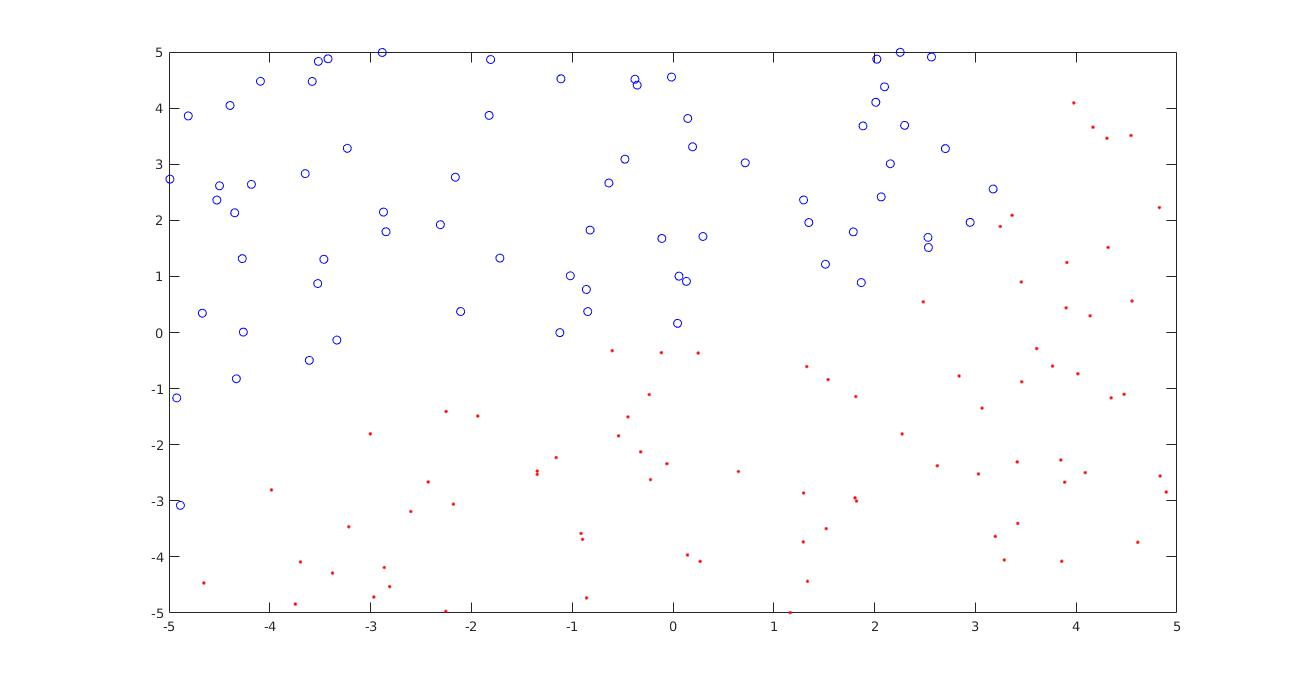
\includegraphics[scale=0.4]{figures/exercise_02_06_01_fig_15.jpg}
        \caption{Training Data X1}
\end{figure}

\begin{center}
\begin{tabular}{ |p{3.5cm}|p{1cm}|p{1cm}|p{1cm}|p{1cm}|p{1cm}|p{1cm}| }
\hline
\multicolumn{7}{|c|}{Testing, Training and Misclassifications Errors of Polynomials of the form $(x^Ty+1)_n$} \\
\hline
               &n=3 & n=5 & n=15 & n=18 & n=20 & n=22 \\
\hline
Iterations & 256 & 474 & 4977 & 30000 & 30000 & 30000 \\
Training error & 0 & 0 & 0 & 0.0133 & 0.0267 & 0.0267 \\
Testing error & 0.0333 & 0.0333 & 0.0533 & 0.0333 & 0.0400 & 0.0533 \\
Misclassifications & 39 & 37 & 31 & 37 & 42 & 40 \\
\hline
\end{tabular}
\end{center}

\newpage
\begin{figure}[h]
    \centering
    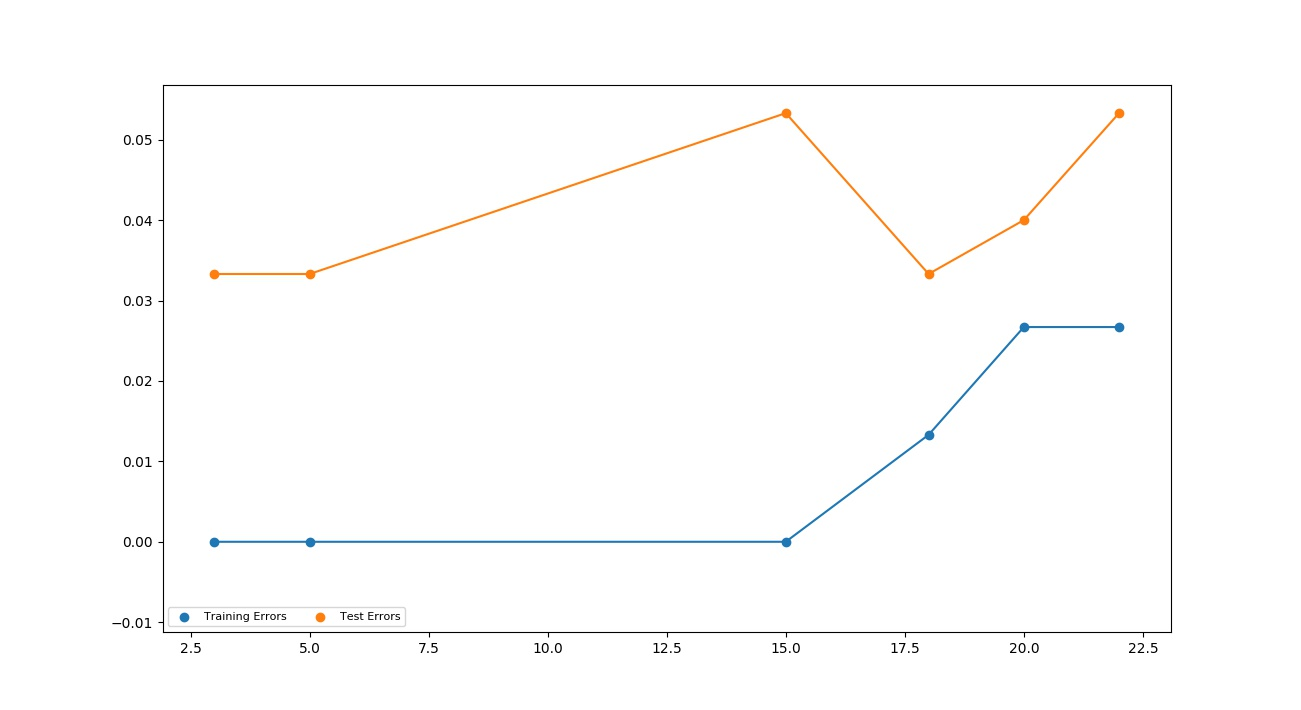
\includegraphics[width=4in,height=3in]{figures/exercise_02_06_01_fig_13.jpg}
    \caption{Testing and Training Errors}
\end{figure}

\newpage

\begin{figure}[h]
\centering
    \begin{subfigure}[h]{0.5\textwidth}
        \centering
        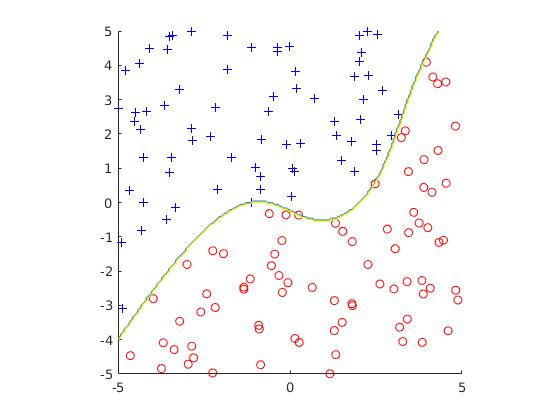
\includegraphics[width=4in,height=3in]{figures/exercise_02_06_01_fig_06.jpg}
        \caption{$(x^Ty+1)^n$ with n=3}
    \end{subfigure}\\
    \begin{subfigure}[h]{0.5\textwidth}
        \centering
        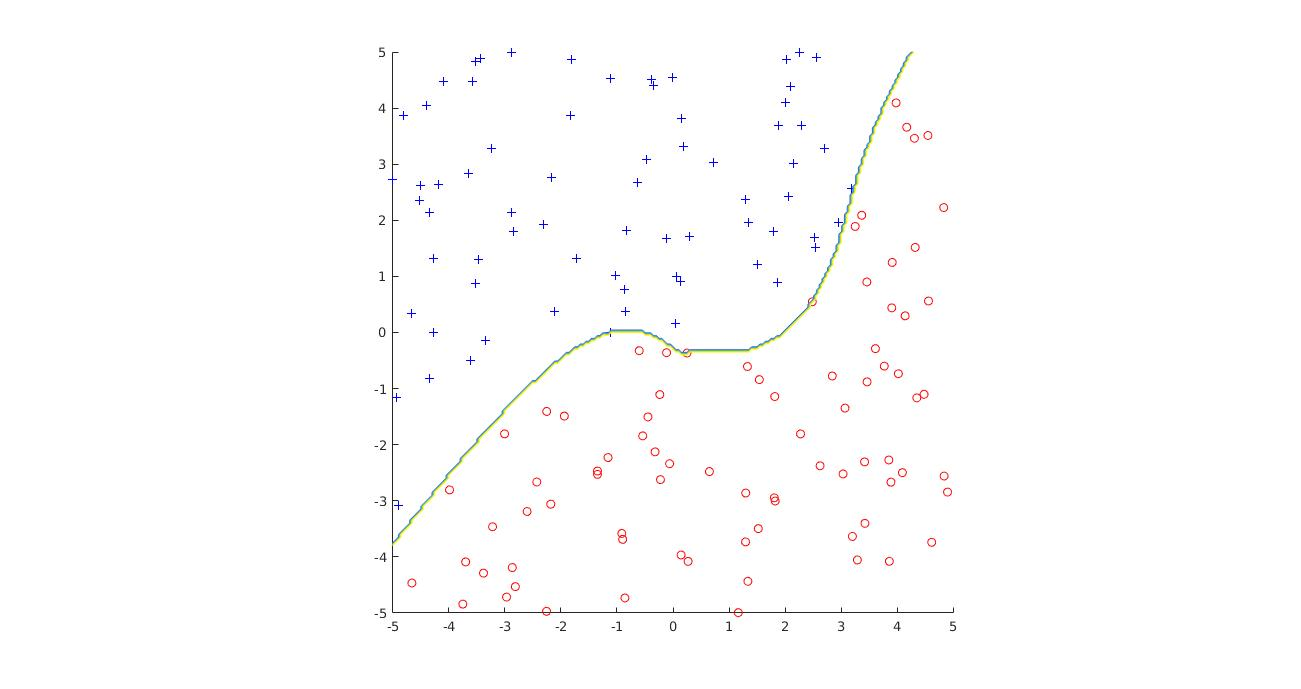
\includegraphics[width=4in,height=3in]{figures/exercise_02_06_01_fig_07.jpg}
        \caption{$(x^Ty+1)^n$ with n=5}
    \end{subfigure}
\end{figure}

\newpage

\begin{figure}[h]
\centering
    \begin{subfigure}[h]{0.5\textwidth}
        \centering
        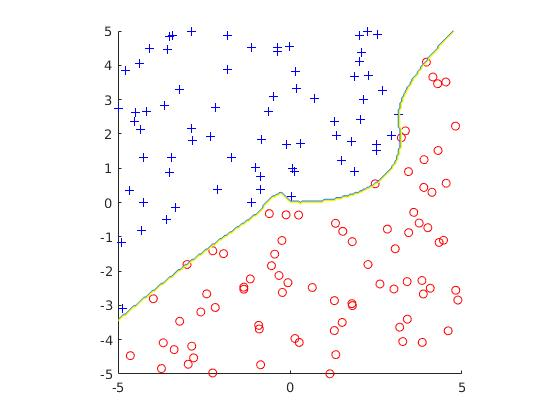
\includegraphics[width=4in,height=3in]{figures/exercise_02_06_01_fig_08.jpg}
        \caption{$(x^Ty+1)^n$ with n=15}
    \end{subfigure}\\
    \begin{subfigure}[h]{0.5\textwidth}
        \centering
        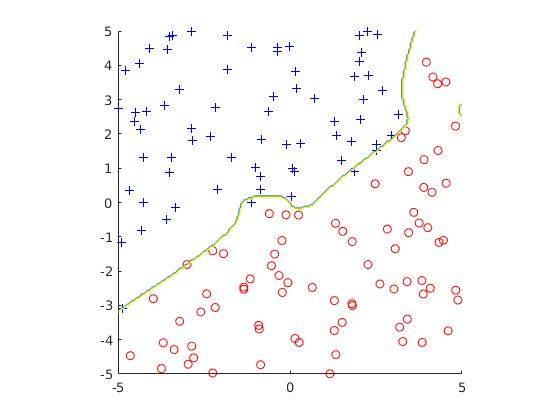
\includegraphics[width=4in,height=3in]{figures/exercise_02_06_01_fig_09.jpg}
        \caption{$(x^Ty+1)^n$ with n=18}
    \end{subfigure}
\end{figure}

\newpage

\begin{figure}[h]
\centering
    \begin{subfigure}[h]{0.5\textwidth}
        \centering
        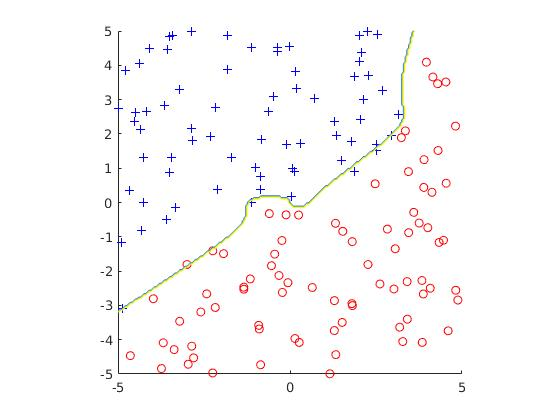
\includegraphics[width=4in,height=3in]{figures/exercise_02_06_01_fig_10.jpg}
        \caption{$(x^Ty+1)^n$ with n=20}
    \end{subfigure}\\
    \begin{subfigure}[h]{0.5\textwidth}
        \centering
        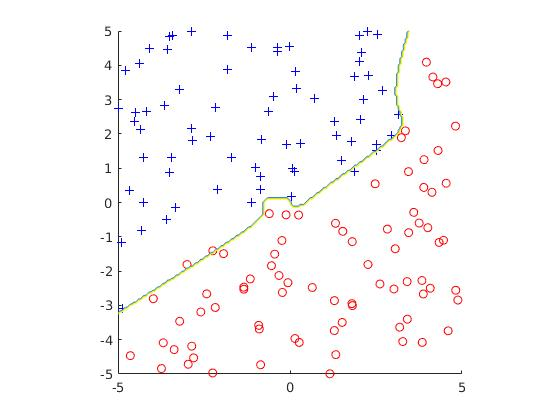
\includegraphics[width=4in,height=3in]{figures/exercise_02_06_01_fig_11.jpg}
        \caption{$(x^Ty+1)^n$ with n=22}
    \end{subfigure}
\end{figure}

\newpage

\begin{center}
\begin{tabular}{ |p{2.5cm}|p{1.2cm}|p{1.2cm}|p{1.2cm}|p{1.2cm}|p{1.2cm}| }
\hline
\multicolumn{6}{|c|}{Testing, Training and Misclassifications Errors of Radial Basis} \\
\hline
               &$\sigma=0.1$ & $\sigma=0.5$ & $\sigma=1$ & $\sigma=1.5$ & $\sigma=2.5$ \\
\hline
Iterations & 4 & 4 & 6 & 18 & 17 \\
Training error & 0 & 0 & 0 & 0 & 0 \\
Testing error & 0.0133 & 0.0133 & 0.0200 & 0.0200 & 0.0267 \\
Misclassifications & 32 & 34 & 33 & 29 & 32 \\
\hline
\end{tabular}
\end{center}

\begin{figure}[h]
    \centering
    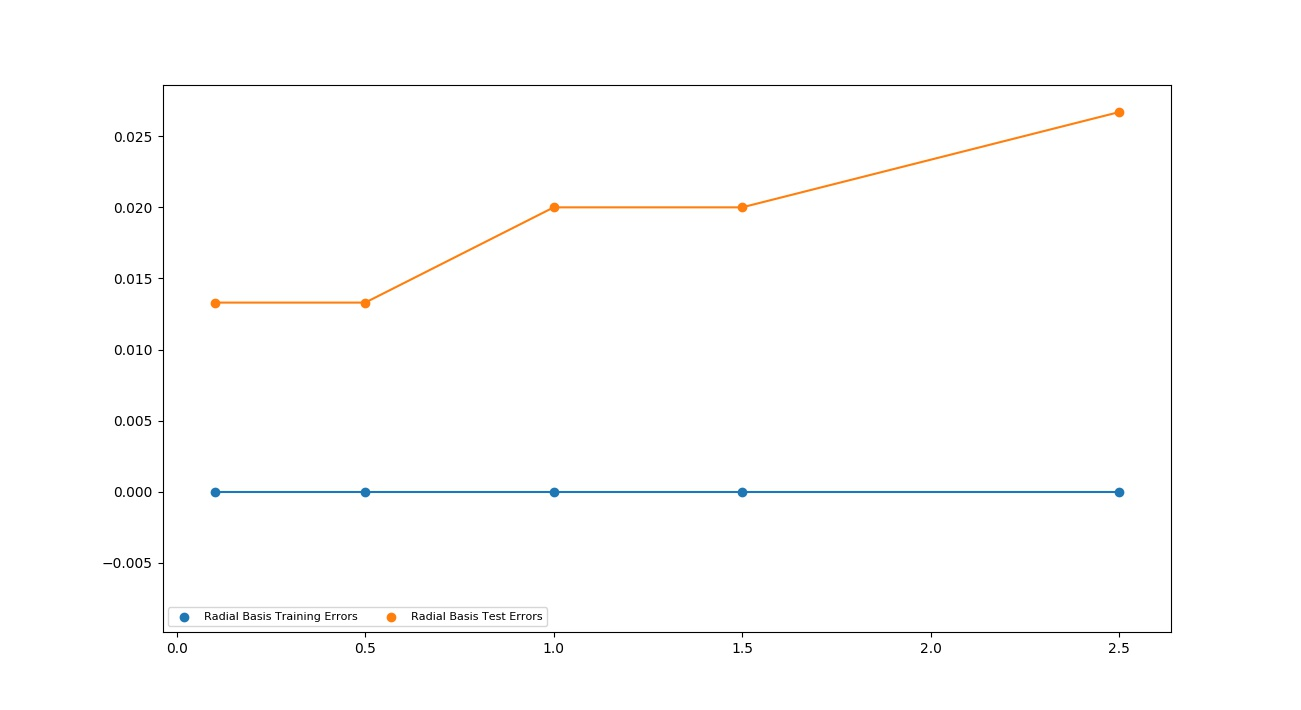
\includegraphics[width=4in,height=3in]{figures/exercise_02_06_01_fig_16.jpg}
    \caption{Training and Test Errors}
\end{figure}

\newpage

\begin{figure}[h]
\centering
    \begin{subfigure}[h]{0.5\textwidth}
        \centering
        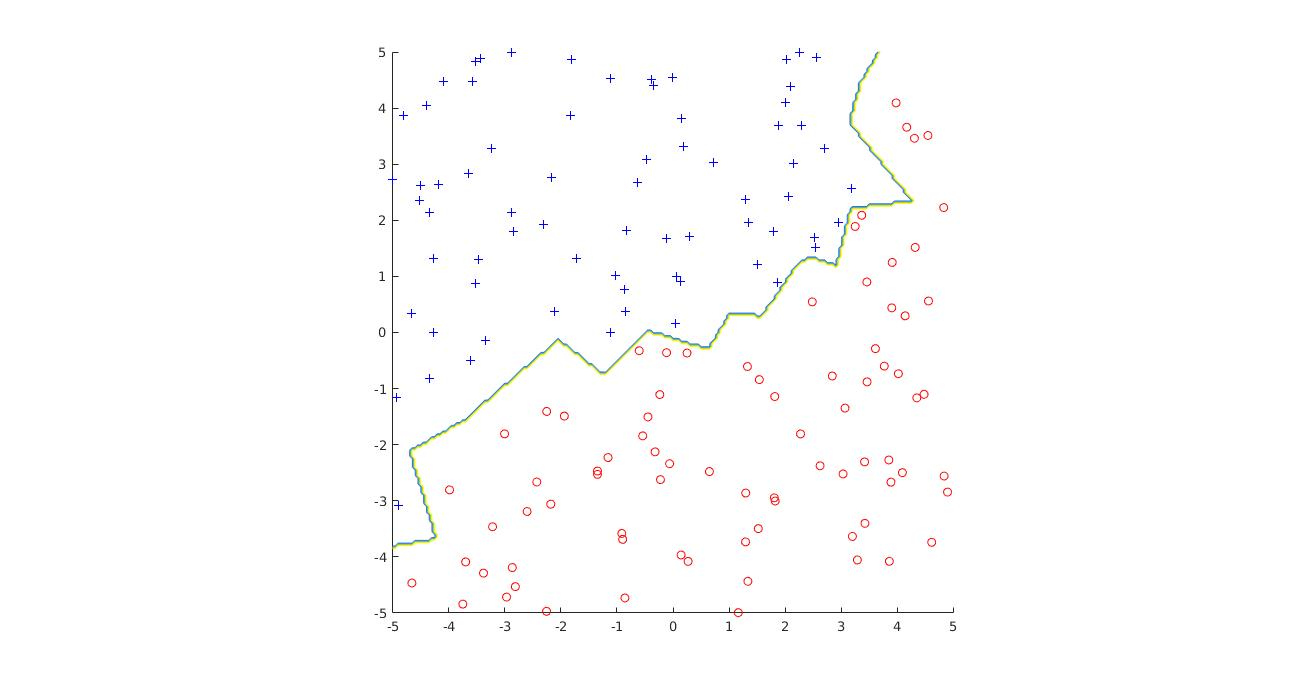
\includegraphics[width=4in,height=3in]{figures/exercise_02_06_01_fig_01.jpg}
        \caption{Radial Basis with $\sigma=0.1$}
    \end{subfigure}\\
    \begin{subfigure}[h]{0.5\textwidth}
        \centering
        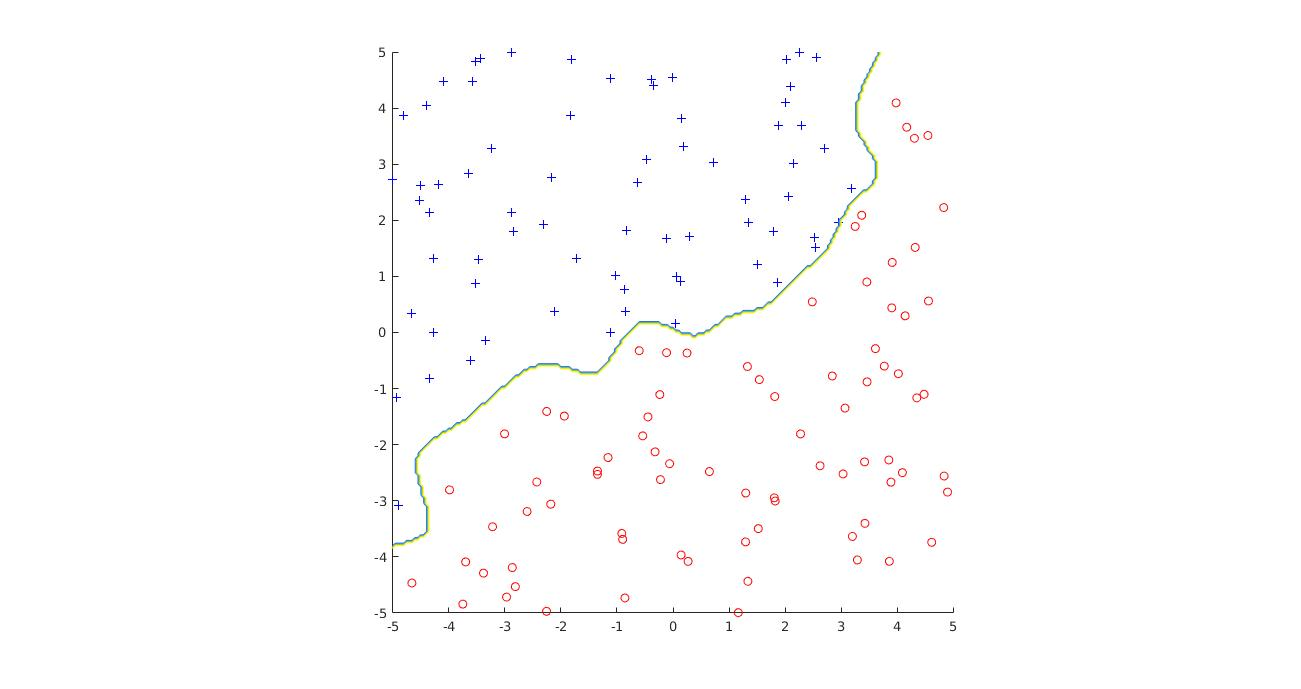
\includegraphics[width=4in,height=3in]{figures/exercise_02_06_01_fig_02.jpg}
        \caption{Radial Basis with $\sigma=0.5$}
    \end{subfigure}
\end{figure}

\newpage

\begin{figure}[ht]
    \centering
    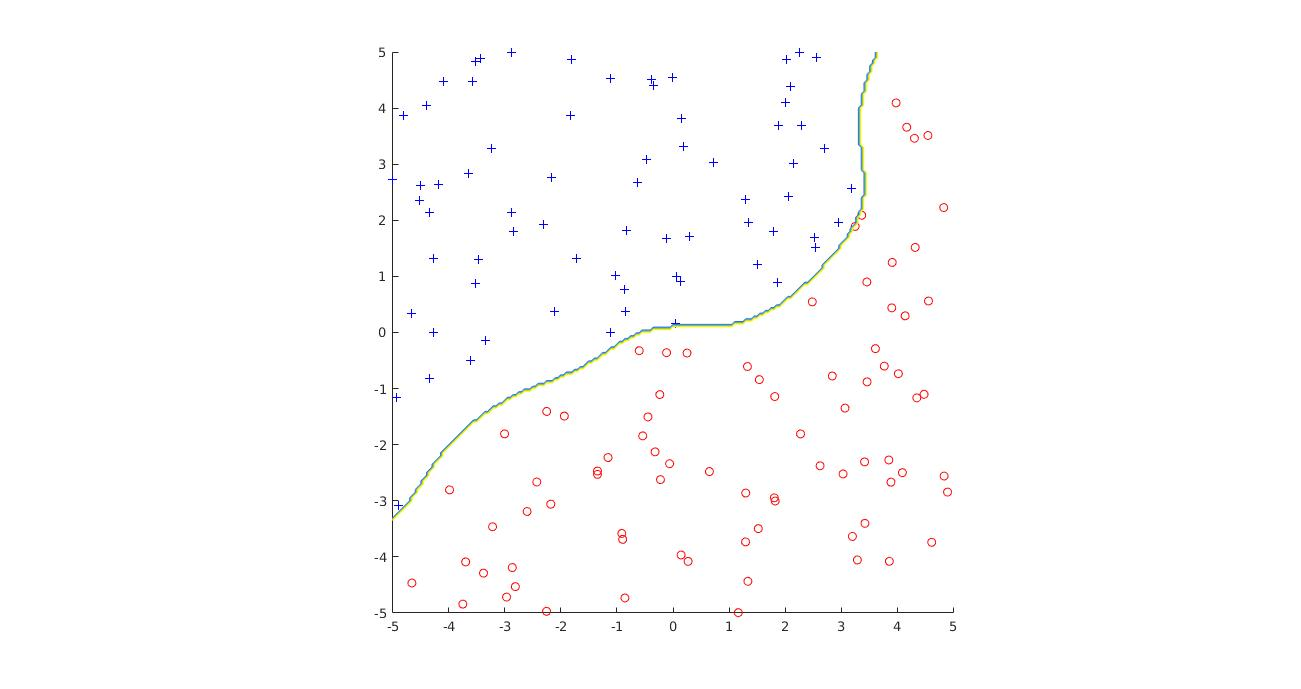
\includegraphics[scale=.2]{figures/exercise_02_06_01_fig_03.jpg}
    \caption{Radial Basis with $\sigma=1$}
\end{figure}
\begin{figure}[ht]
    \centering
    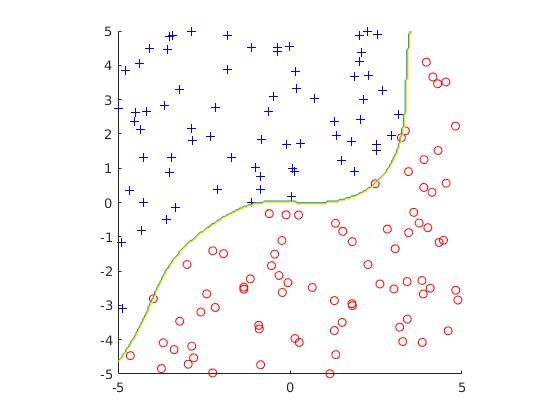
\includegraphics[scale=.3]{figures/exercise_02_06_01_fig_04.jpg}
    \caption{Radial Basis with $\sigma=1.5$}
\end{figure}

\newpage

\begin{figure}[ht]
    \centering
    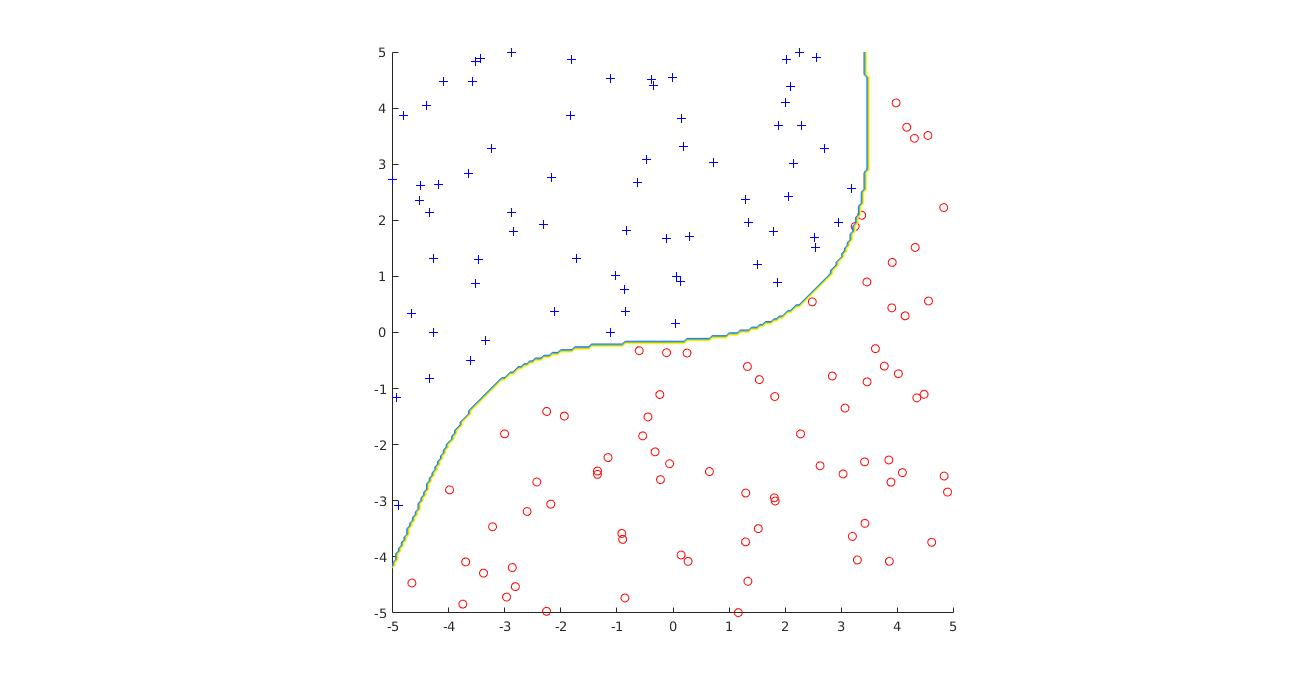
\includegraphics[scale=.4]{figures/exercise_02_06_01_fig_05.jpg}
    \caption{Radial Basis with $\sigma=2.5$}
\end{figure}

\end{homeworkProblem}
%-------------END PROBLEM 2--------------------------------------------------------------

%----------------------------------------------------------------------------------------
%	PROBLEM 3
%----------------------------------------------------------------------------------------

\newpage
\begin{homeworkProblem}
\maketitle
\subsection{Exercise 2.8.2}
\matlabscript{mfiles/exercise_02_08_02}{Source codes}

\newpage
\subsubsection{$\sigma=2$}

\begin{center}
\begin{tabular}{ |p{3.5cm}|p{1.2cm}|p{1.2cm}| }
\hline
\multicolumn{3}{|c|}{Test and Training Errors with $\sigma=2$} \\
\hline
No.Hidden Layers & Training & Test \\
\hline
7 & 0.1222 & 0.1111\\
8 & 0.1611 & 0.1611\\
10 & 0.0722 & 0.1333\\
14 & 0.0111 & 0.0500\\
16 & 0.0167 & 0.0444\\
20 & 0.0056 & 0.0611\\
32 & 0.0056 & 0.0389\\
40 & 0.0111 & 0.0611\\
\hline
\end{tabular}
\end{center}

\newpage

\begin{figure}[h]
        \centering
        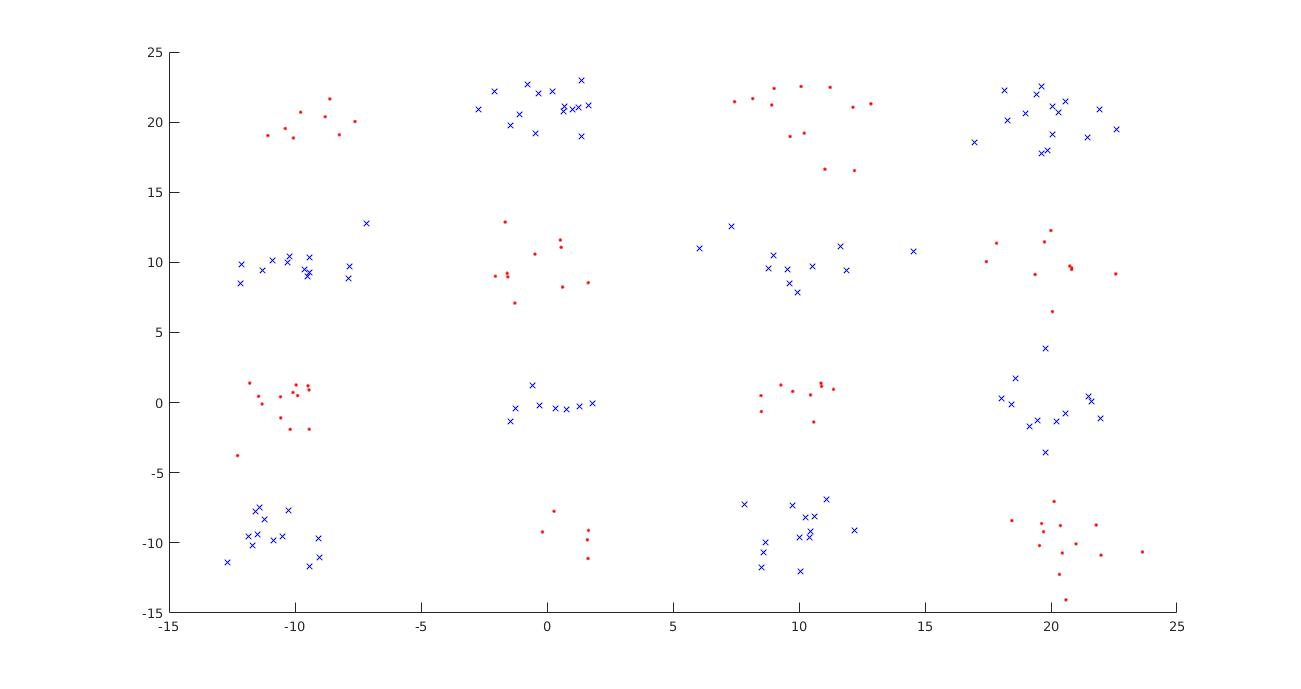
\includegraphics[scale=0.3]{figures/exercise_02_08_02_fig_26.jpg}
        \caption{Training Data X1 with $\sigma=2$}
\end{figure}

\newpage

\begin{figure}[ht]
    \begin{subfigure}[h]{0.5\textwidth}
        \centering
        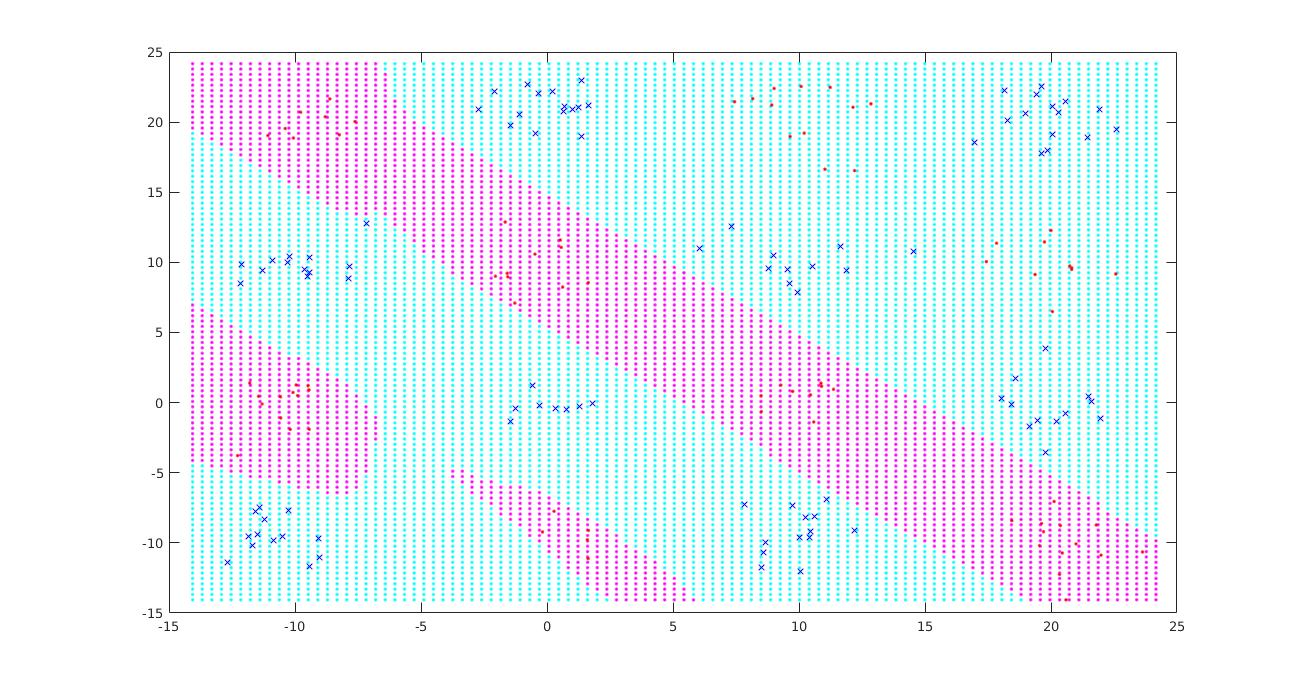
\includegraphics[scale=.3]{figures/exercise_02_08_02_fig_48.jpg}
        \caption{No.Hidden Layers = 7}
    \end{subfigure}\\
    \begin{subfigure}[h]{0.5\textwidth}
        \centering
        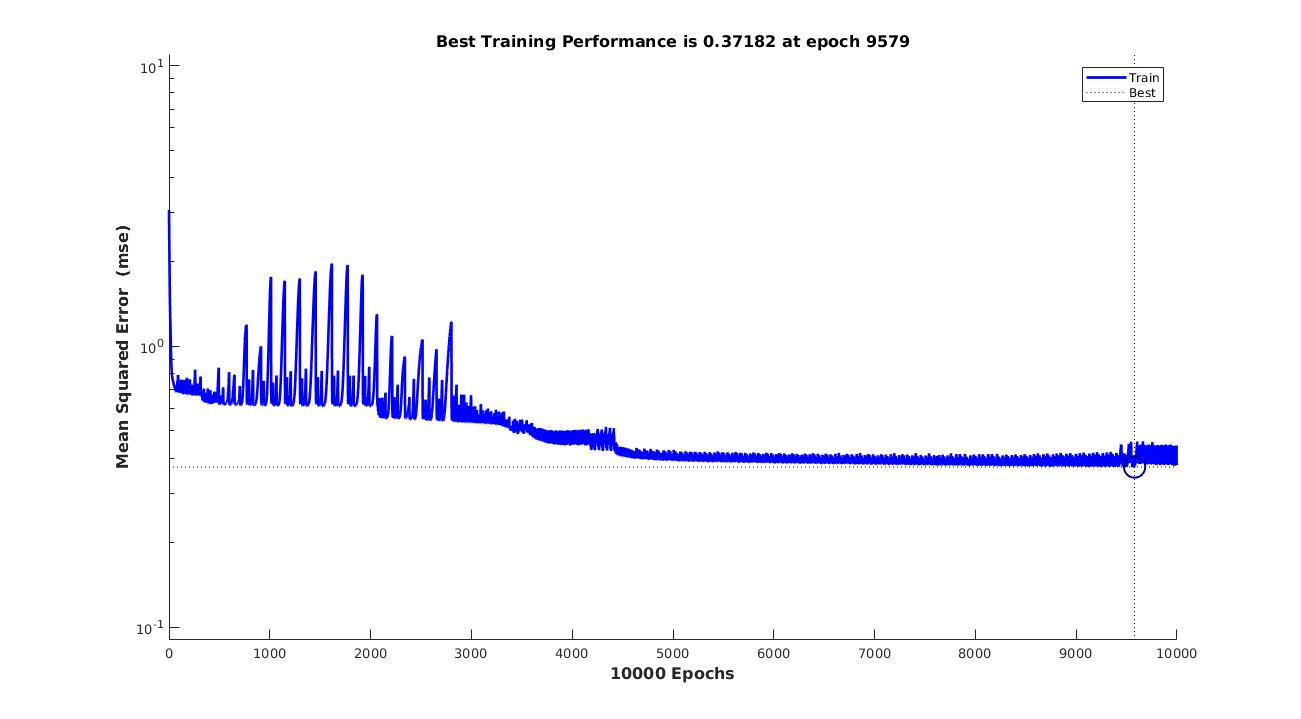
\includegraphics[scale=.3]{figures/exercise_02_08_02_fig_49.jpg}
        \caption{No.Hidden Layers = 7}
    \end{subfigure}\\
\end{figure}

\newpage

\begin{figure}[ht]
    \begin{subfigure}[h]{0.5\textwidth}
        \centering
        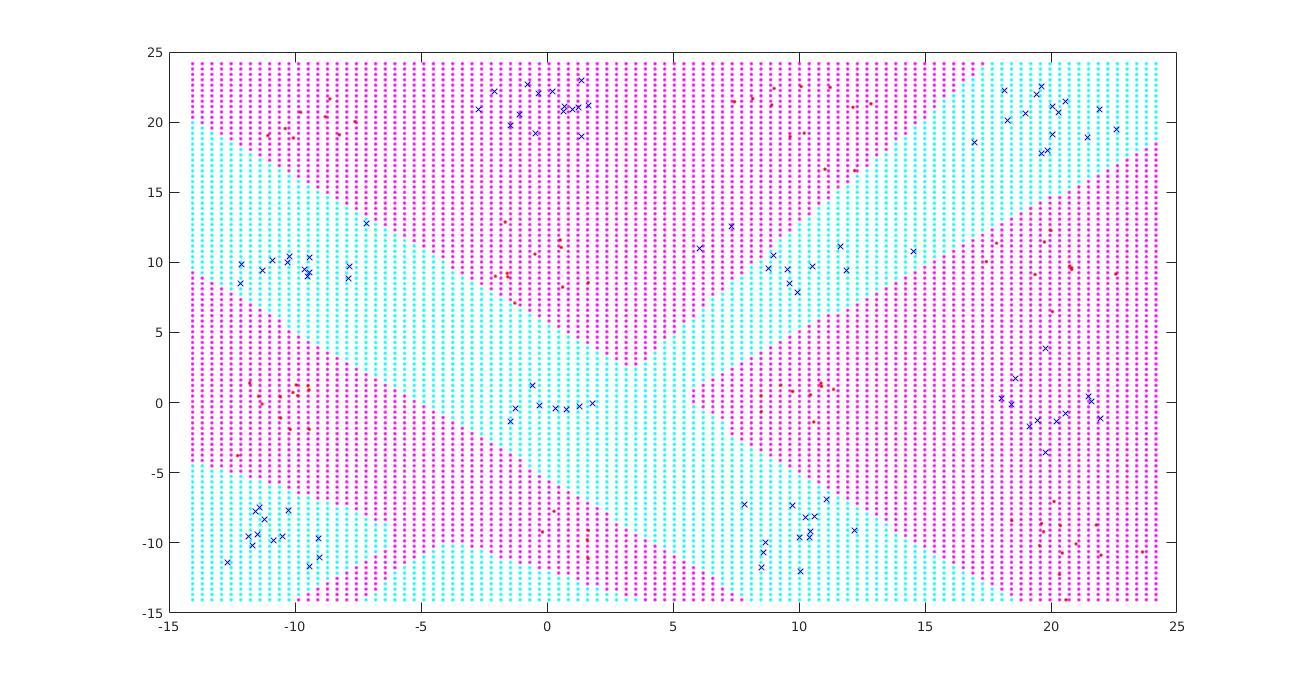
\includegraphics[scale=.3]{figures/exercise_02_08_02_fig_45.jpg}
        \caption{No.Hidden Layers = 8}
    \end{subfigure}\\
    \begin{subfigure}[h]{0.5\textwidth}
        \centering
        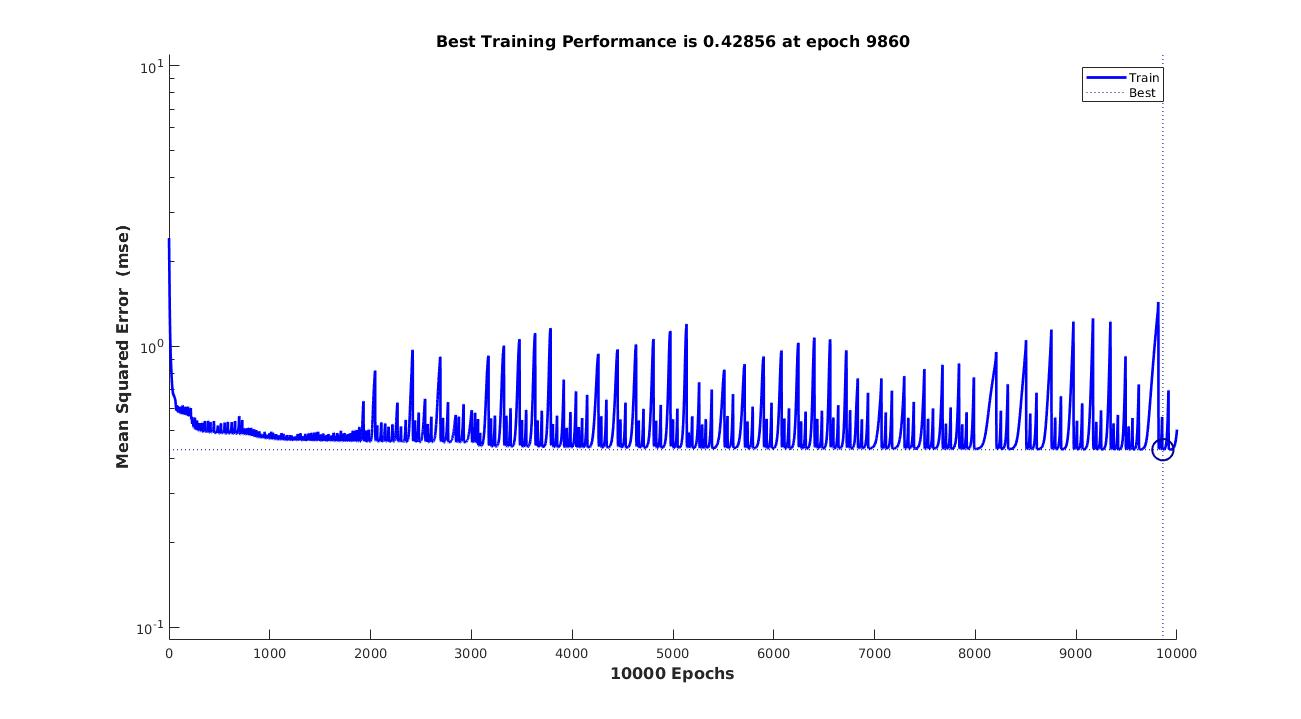
\includegraphics[scale=.3]{figures/exercise_02_08_02_fig_46.jpg}
        \caption{No.Hidden Layers = 8}
    \end{subfigure}\\
\end{figure}

\newpage

\begin{figure}[ht]
    \begin{subfigure}[h]{0.5\textwidth}
        \centering
        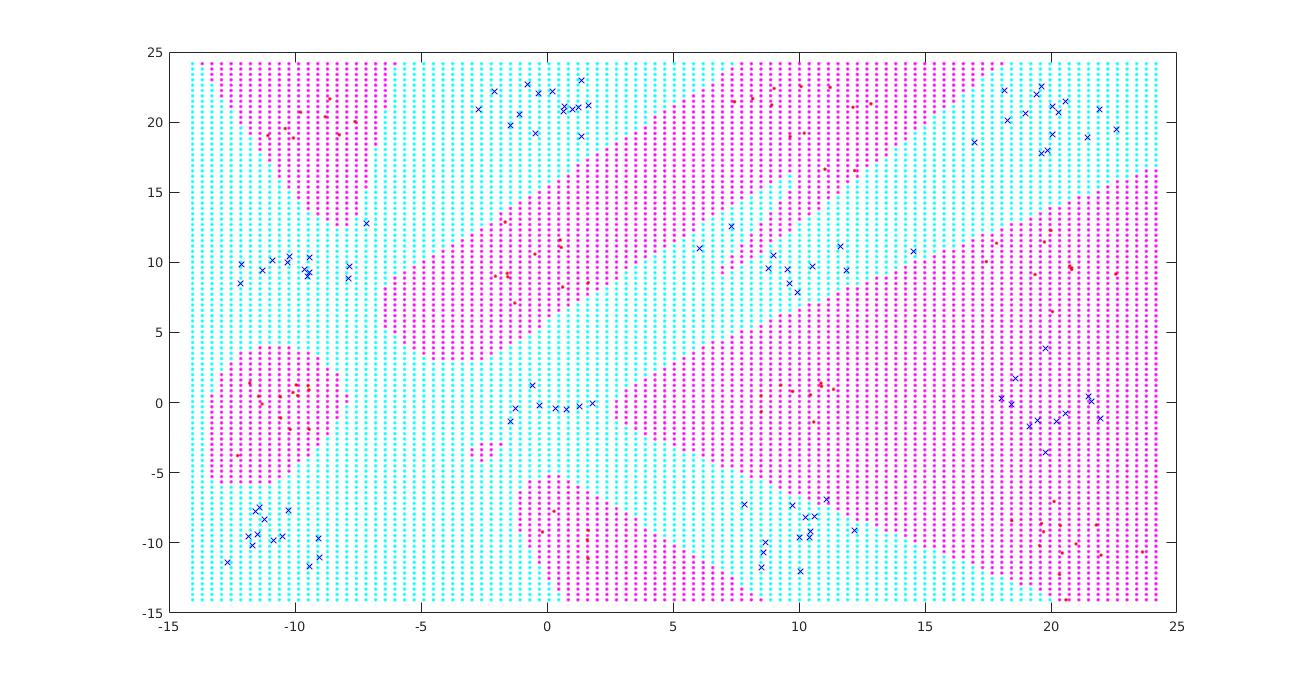
\includegraphics[scale=.3]{figures/exercise_02_08_02_fig_42.jpg}
        \caption{No.Hidden Layers = 10}
    \end{subfigure}\\
    \begin{subfigure}[h]{0.5\textwidth}
        \centering
        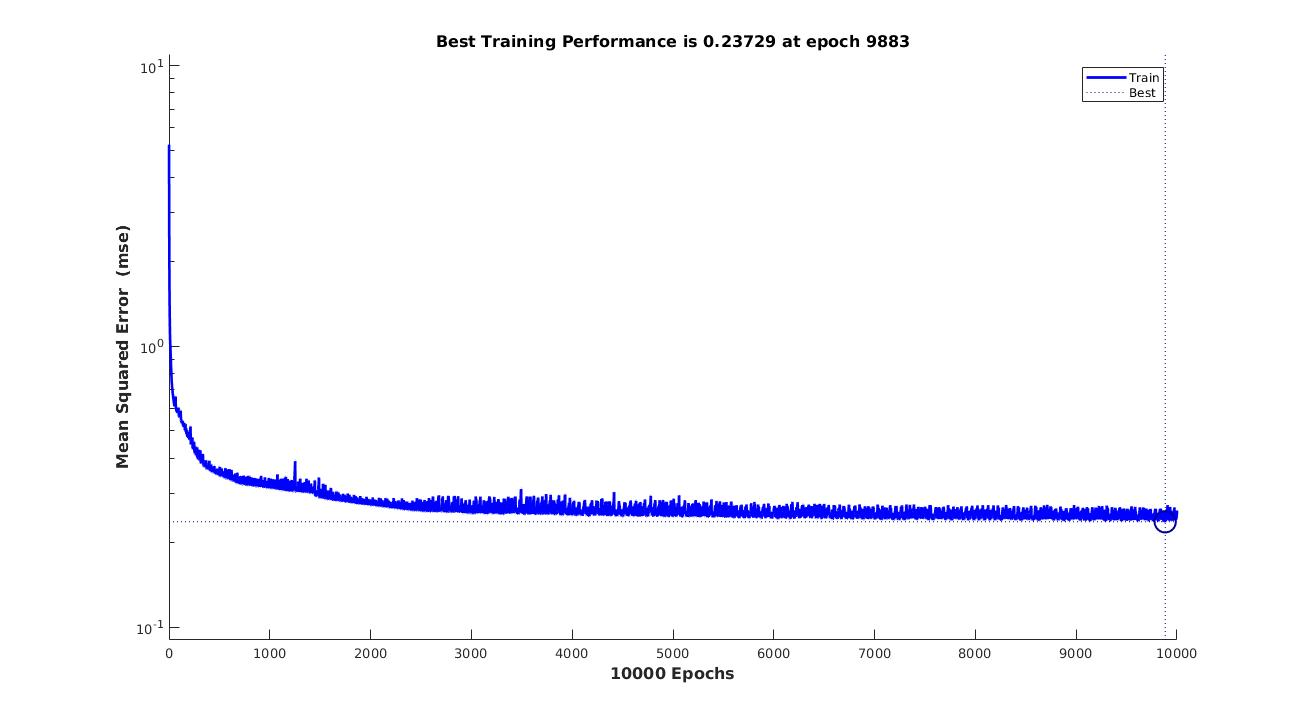
\includegraphics[scale=.3]{figures/exercise_02_08_02_fig_43.jpg}
        \caption{No.Hidden Layers = 10}
    \end{subfigure}\\
\end{figure}

\newpage

\begin{figure}[ht]
    \begin{subfigure}[h]{0.5\textwidth}
        \centering
        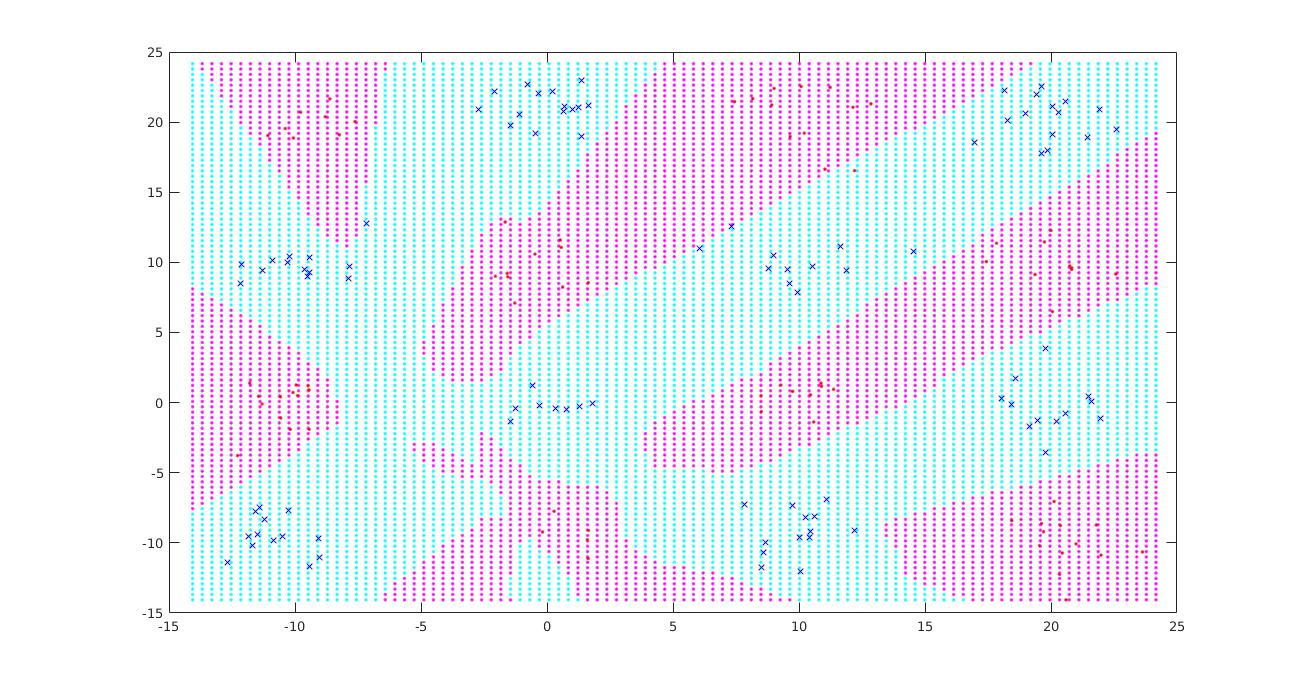
\includegraphics[scale=.3]{figures/exercise_02_08_02_fig_39.jpg}
        \caption{No.Hidden Layers = 14}
    \end{subfigure}\\
    \begin{subfigure}[h]{0.5\textwidth}
        \centering
        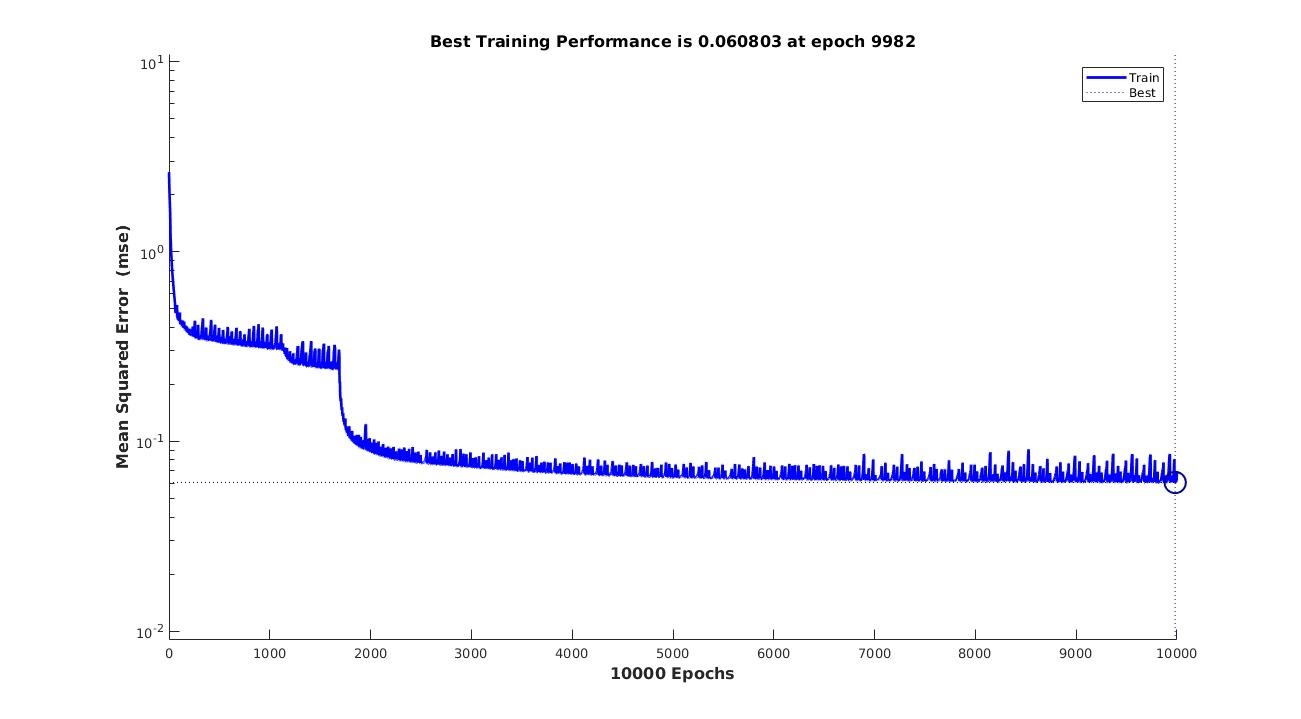
\includegraphics[scale=.3]{figures/exercise_02_08_02_fig_40.jpg}
        \caption{No.Hidden Layers = 14}
    \end{subfigure}\\
\end{figure}

\newpage

\begin{figure}[ht]
    \begin{subfigure}[h]{0.5\textwidth}
        \centering
        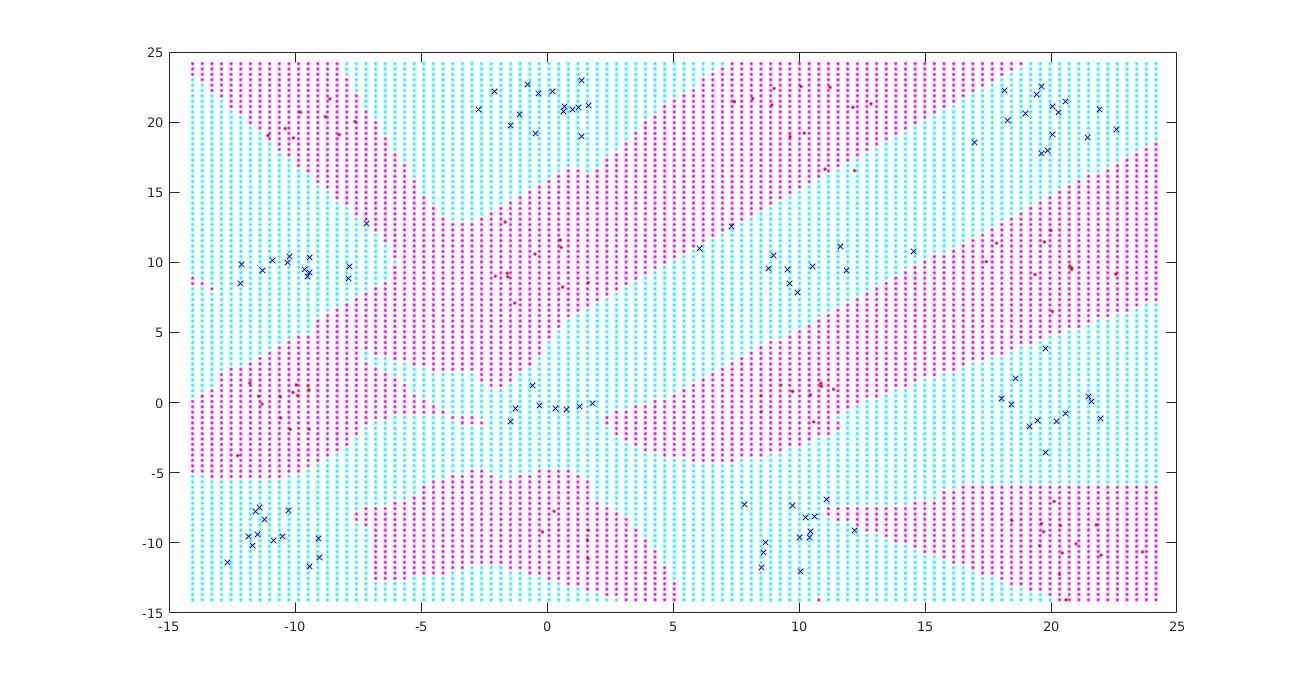
\includegraphics[scale=.3]{figures/exercise_02_08_02_fig_36.jpg}
        \caption{No.Hidden Layers = 16}
    \end{subfigure}\\
    \begin{subfigure}[h]{0.5\textwidth}
        \centering
        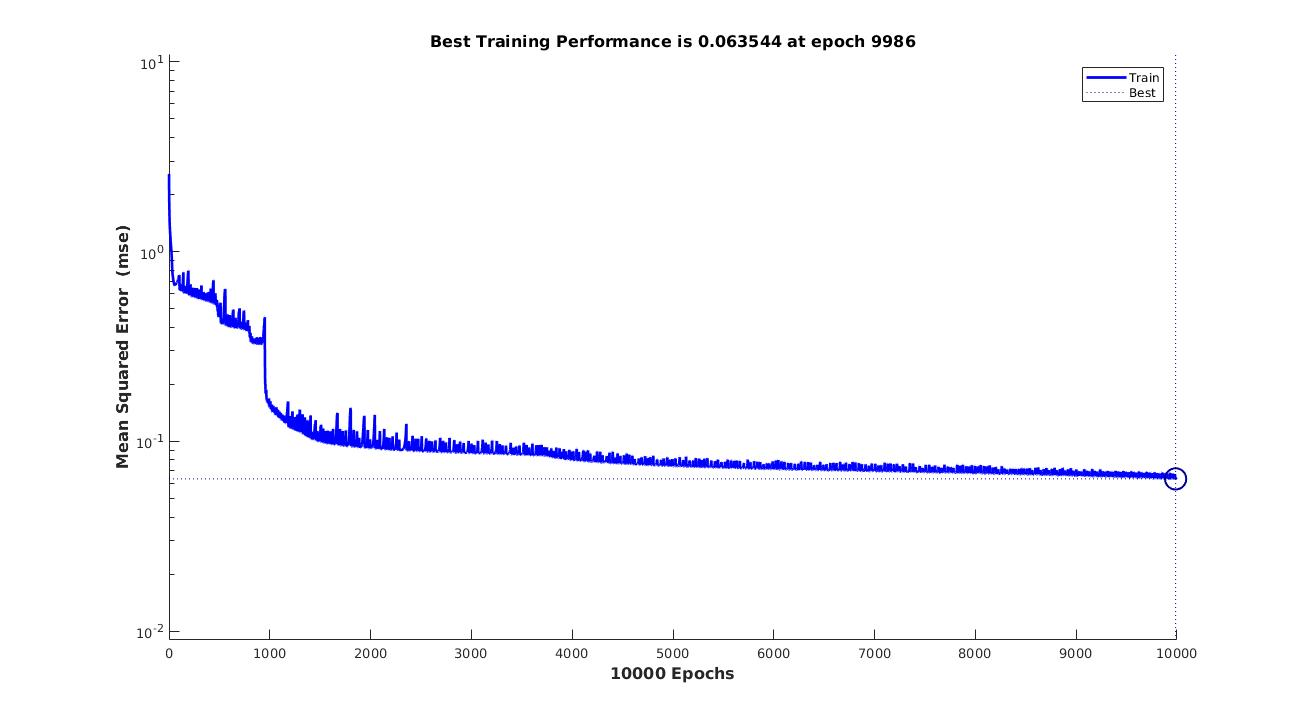
\includegraphics[scale=.3]{figures/exercise_02_08_02_fig_37.jpg}
        \caption{No.Hidden Layers = 16}
    \end{subfigure}\\
\end{figure}

\newpage

\begin{figure}[ht]
    \begin{subfigure}[h]{0.5\textwidth}
        \centering
        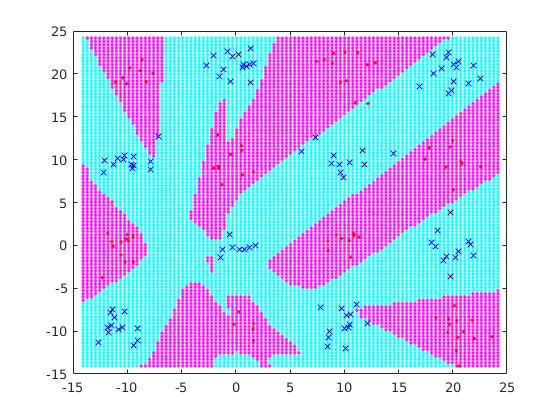
\includegraphics[scale=.5]{figures/exercise_02_08_02_fig_33.jpg}
        \caption{No.Hidden Layers = 20}
    \end{subfigure}\\
    \begin{subfigure}[h]{0.5\textwidth}
        \centering
        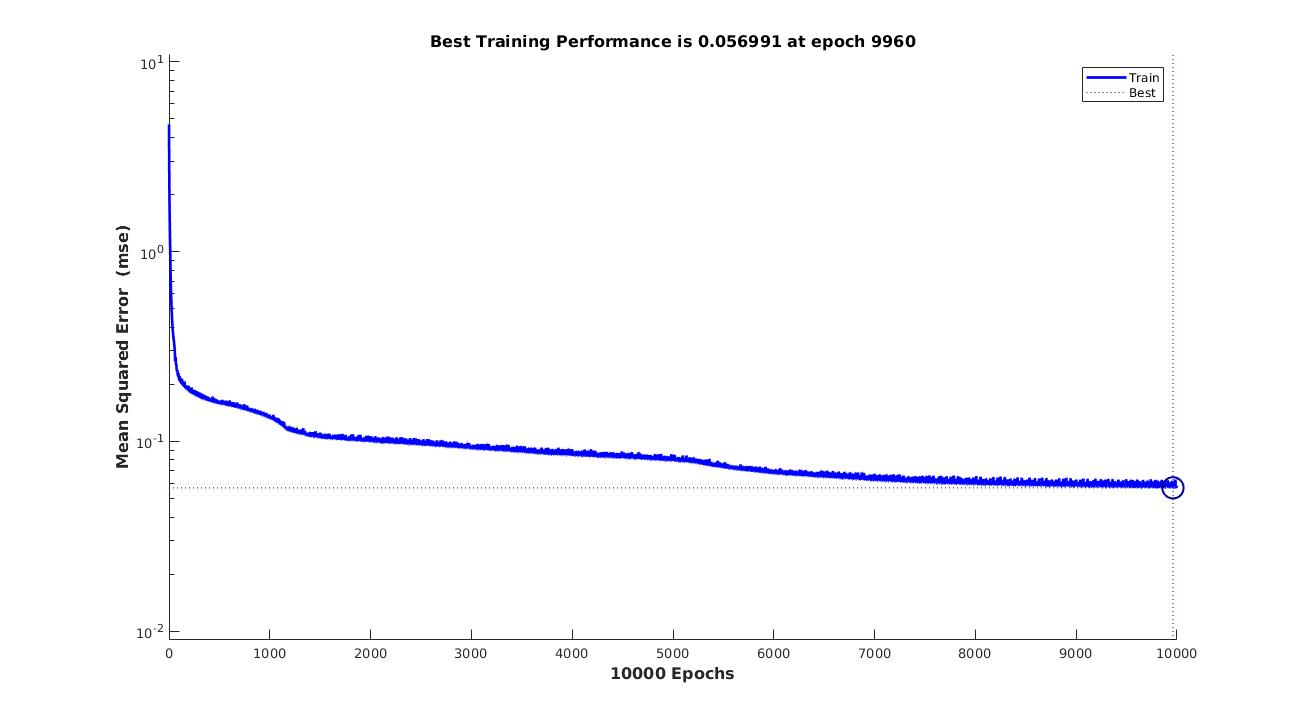
\includegraphics[scale=.2]{figures/exercise_02_08_02_fig_34.jpg}
        \caption{No.Hidden Layers = 20}
    \end{subfigure}\\
\end{figure}

\newpage

\begin{figure}[ht]
    \begin{subfigure}[h]{0.5\textwidth}
        \centering
        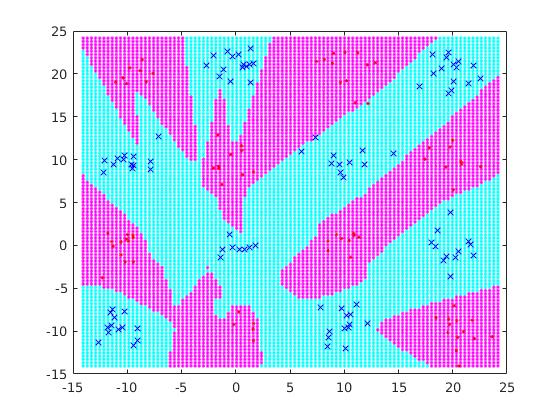
\includegraphics[scale=.5]{figures/exercise_02_08_02_fig_30.jpg}
        \caption{No.Hidden Layers = 32}
    \end{subfigure}\\
    \begin{subfigure}[h]{0.5\textwidth}
        \centering
        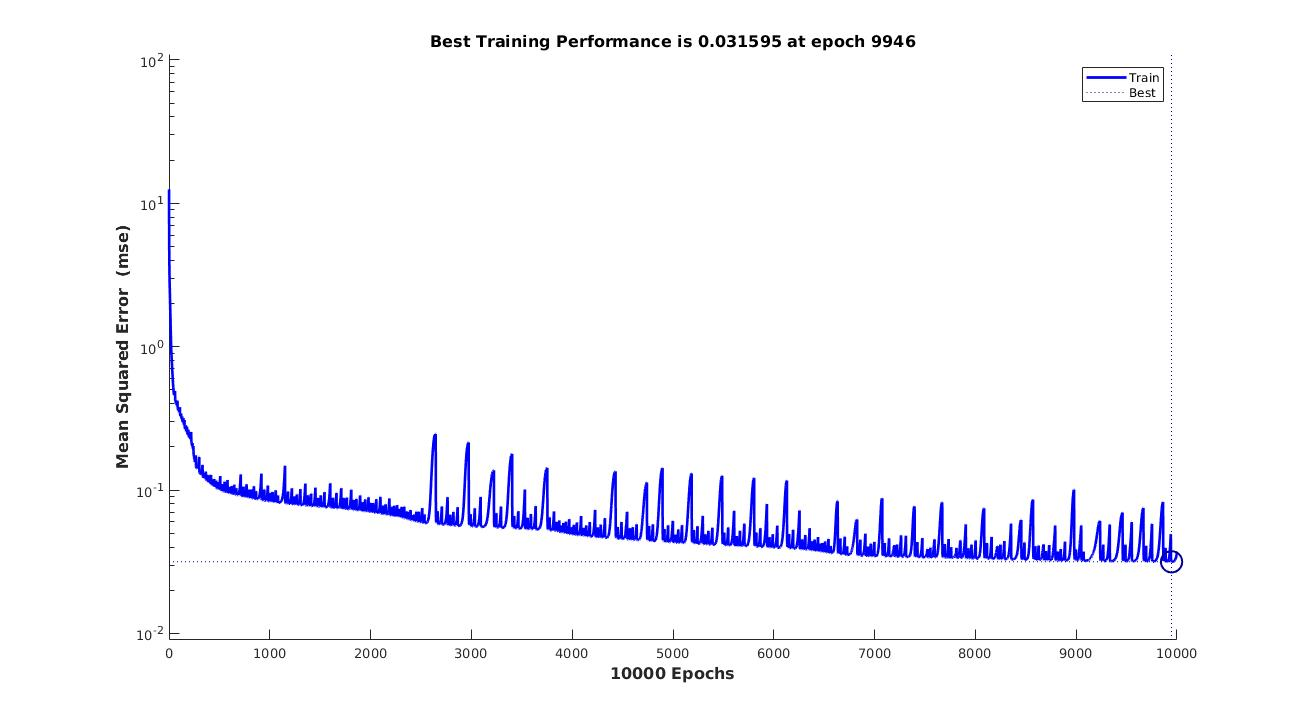
\includegraphics[scale=.2]{figures/exercise_02_08_02_fig_31.jpg}
        \caption{No.Hidden Layers = 32}
    \end{subfigure}\\
\end{figure}

\newpage

\begin{figure}[ht]
    \begin{subfigure}[h]{0.5\textwidth}
        \centering
        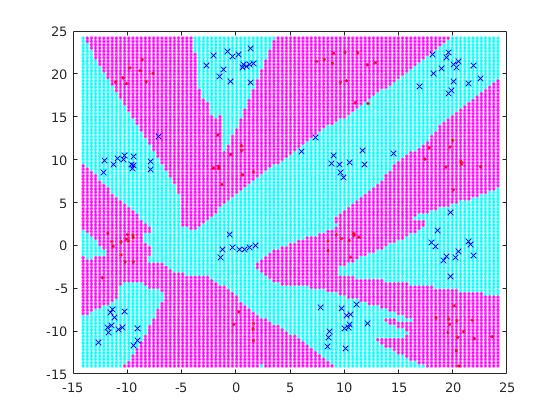
\includegraphics[scale=.5]{figures/exercise_02_08_02_fig_27.jpg}
        \caption{No.Hidden Layers = 40}
    \end{subfigure}\\
    \begin{subfigure}[h]{0.5\textwidth}
        \centering
        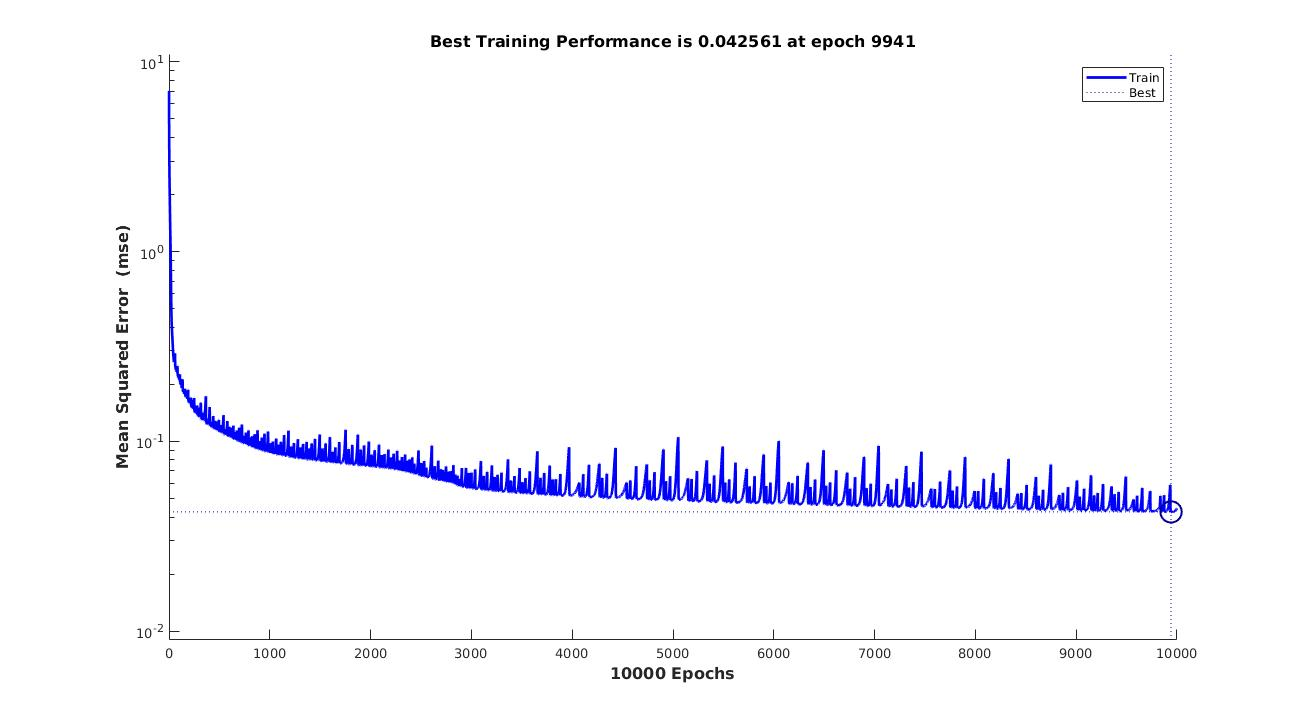
\includegraphics[scale=.2]{figures/exercise_02_08_02_fig_28.jpg}
        \caption{No.Hidden Layers = 40}
    \end{subfigure}\\
\end{figure}

\newpage

\begin{figure}[ht]
    \centering
    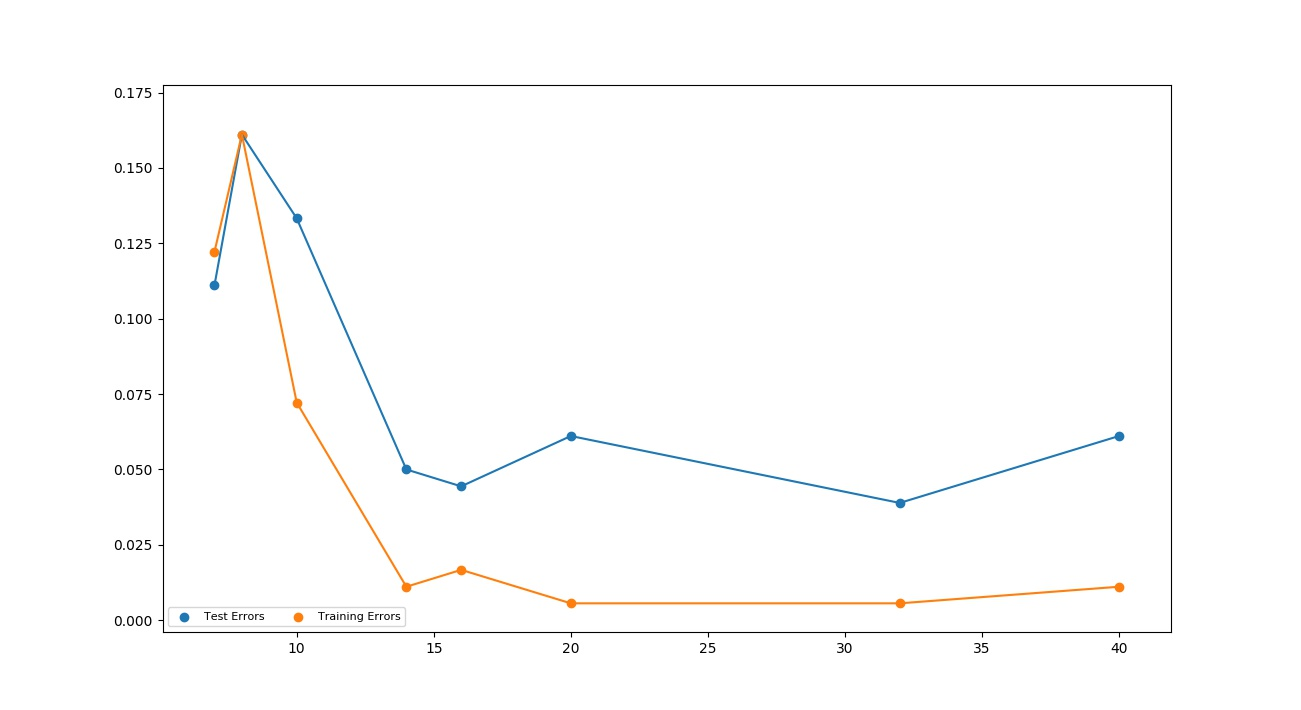
\includegraphics[scale=.3]{figures/exercise_02_08_02_fig_76.jpg}
    \caption{Training and Test Errors with $\sigma=2$}
\end{figure}

\newpage
\subsubsection{$\sigma=3$}

\begin{center}
\begin{tabular}{ |p{4cm}|p{1.2cm}|p{1.2cm}| }
\hline
\multicolumn{3}{|c|}{Test and Training Errors with $\sigma=3$} \\
\hline
No.Hidden Layers & Training & Test \\
\hline
7 & 0.1278 & 0.1222\\
8 & 0.1778 & 0.2222\\
10 & 0.1000 & 0.1778\\
14 & 0.00944 & 0.1333\\
16 & 0.0833 & 0.1222\\
20 & 0.0222 & 0.1389\\
32 & 0.0167 & 0.0778\\
40 & 0.0167 & 0.1222\\
\hline
\end{tabular}
\end{center}

\newpage
\begin{figure}[h]
        \centering
        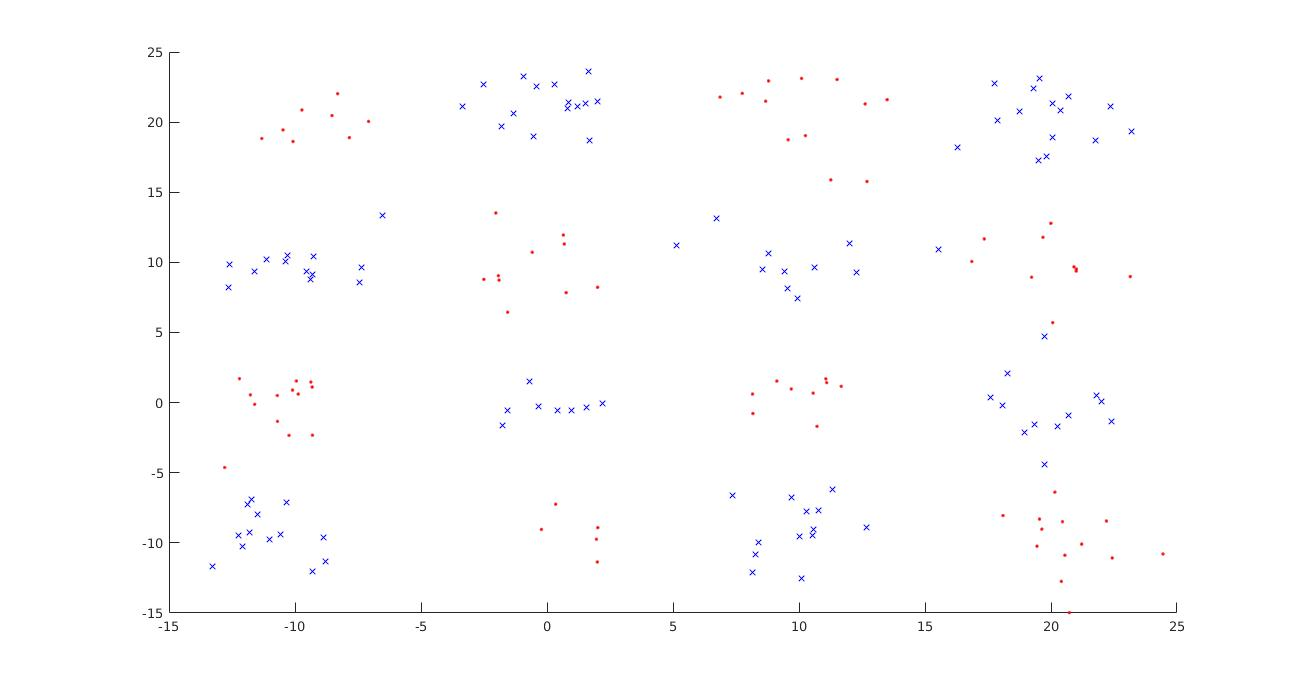
\includegraphics[scale=0.3]{figures/exercise_02_08_02_fig_51.jpg}
        \caption{Training Data X1 with $\sigma=3$}
\end{figure}

\newpage

\begin{figure}[ht]
    \begin{subfigure}[h]{0.5\textwidth}
        \centering
        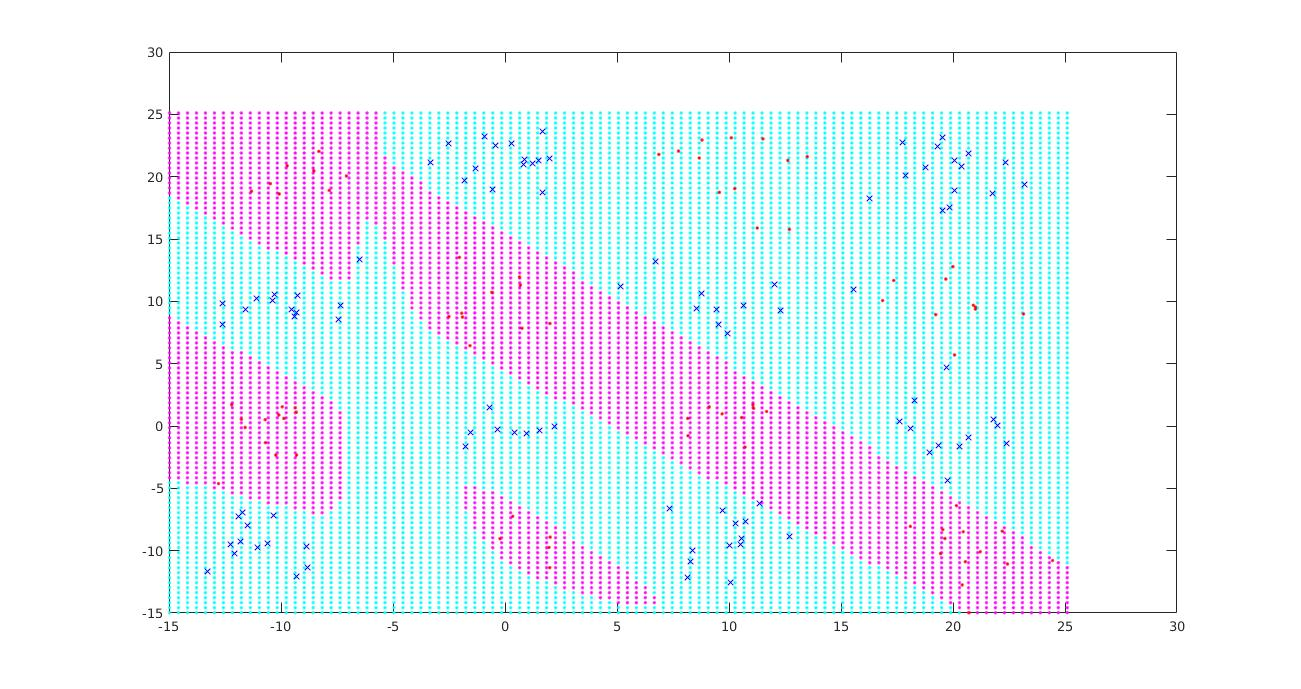
\includegraphics[scale=.3]{figures/exercise_02_08_02_fig_52.jpg}
        \caption{No.Hidden Layers = 7}
    \end{subfigure}\\
    \begin{subfigure}[h]{0.5\textwidth}
        \centering
        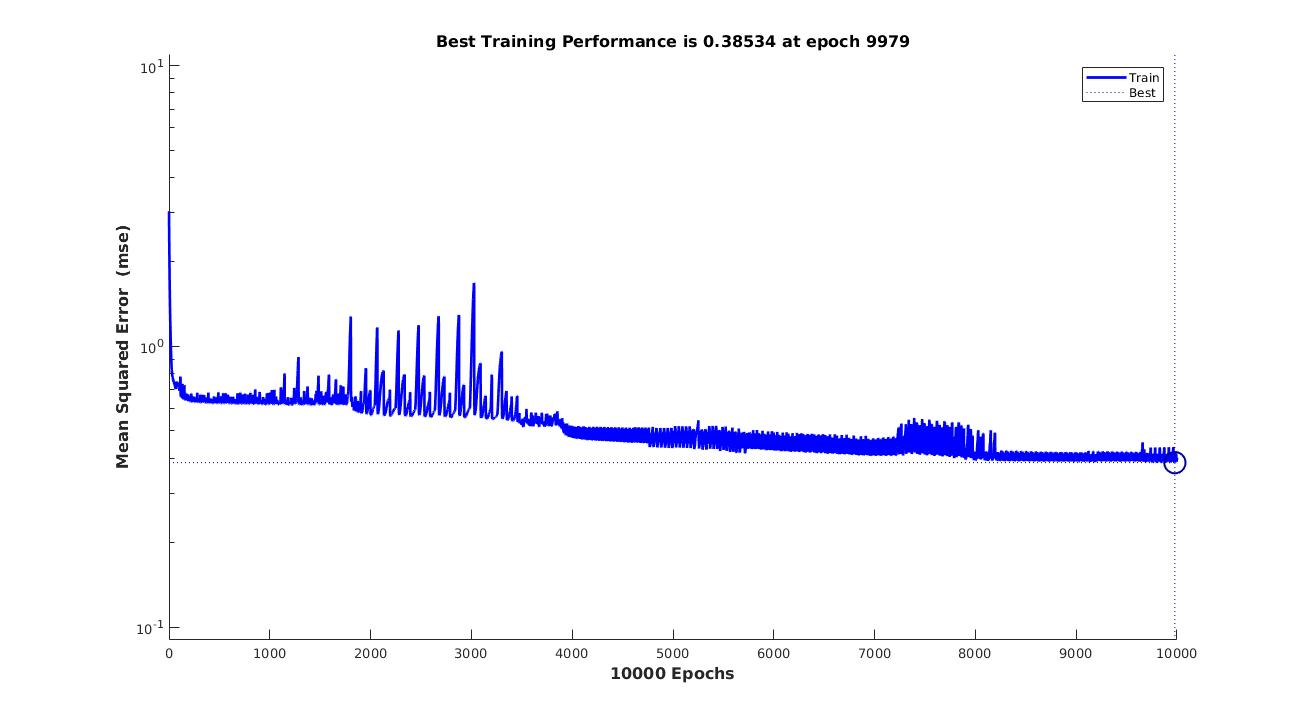
\includegraphics[scale=.3]{figures/exercise_02_08_02_fig_53.jpg}
        \caption{No.Hidden Layers = 7}
    \end{subfigure}\\
\end{figure}

\newpage

\begin{figure}[ht]
    \begin{subfigure}[h]{0.5\textwidth}
        \centering
        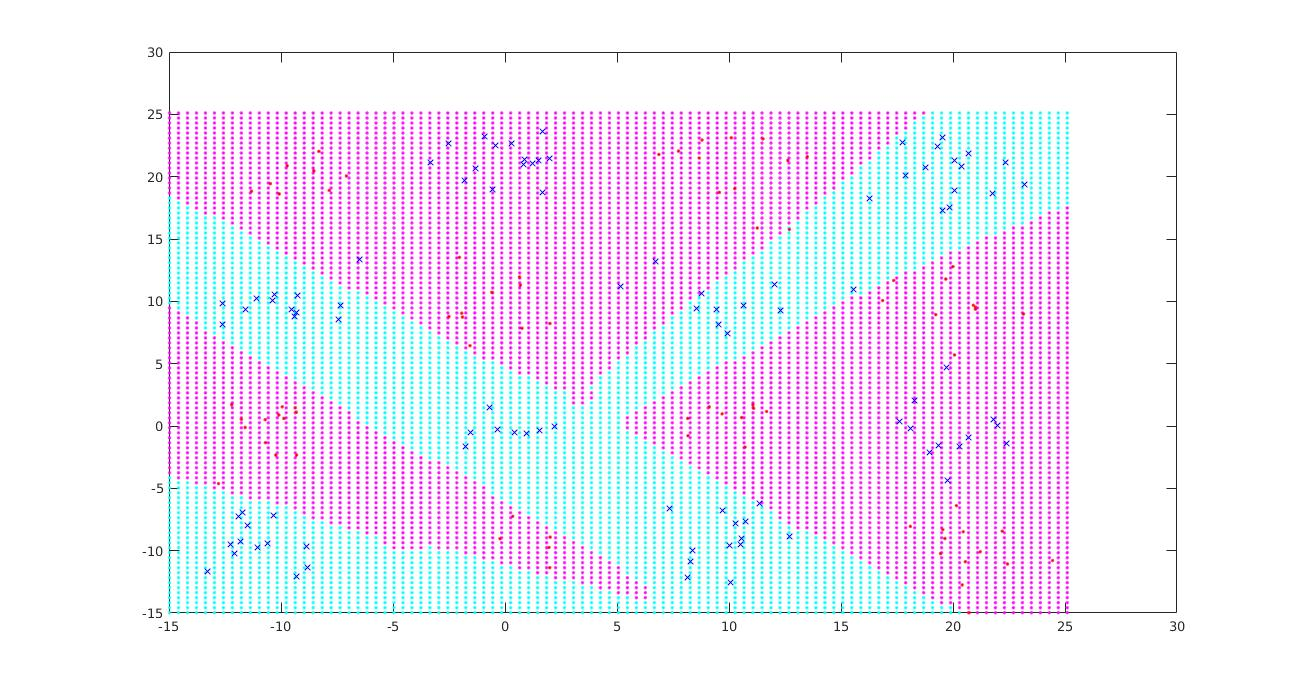
\includegraphics[scale=.3]{figures/exercise_02_08_02_fig_55.jpg}
        \caption{No.Hidden Layers = 8}
    \end{subfigure}\\
    \begin{subfigure}[h]{0.5\textwidth}
        \centering
        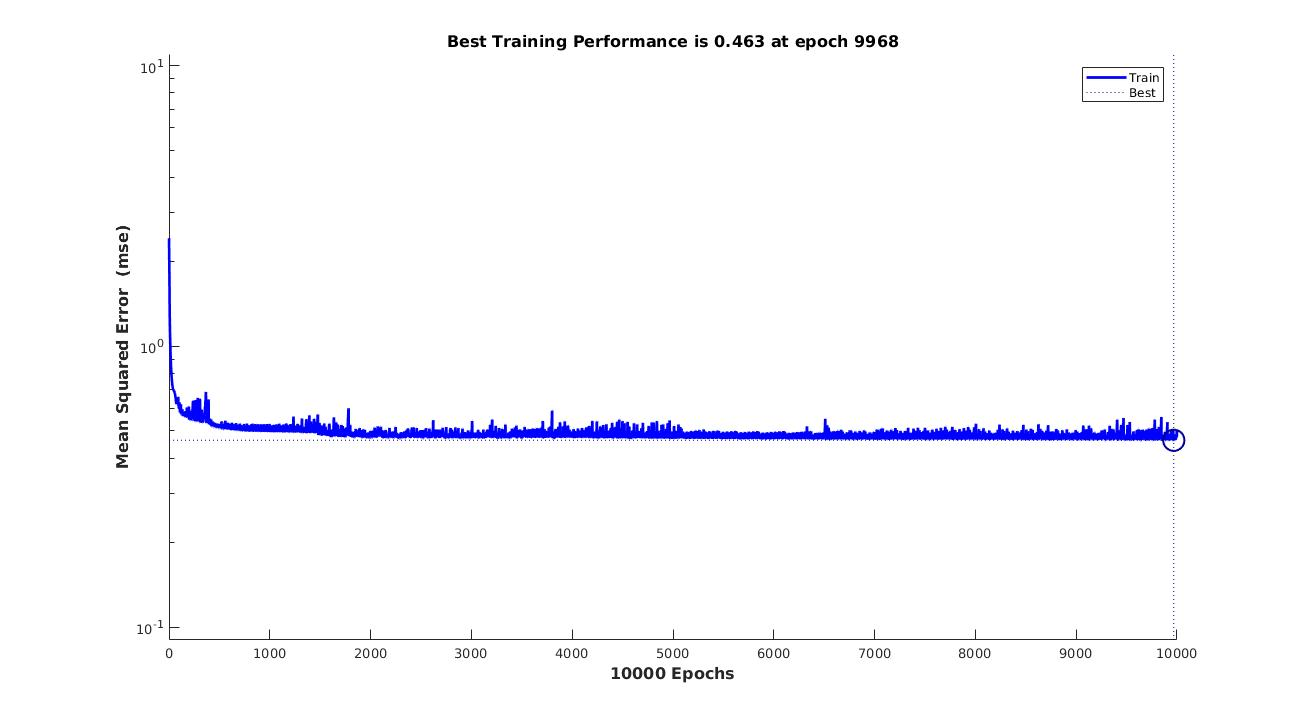
\includegraphics[scale=.3]{figures/exercise_02_08_02_fig_56.jpg}
        \caption{No.Hidden Layers = 8}
    \end{subfigure}\\
\end{figure}

\newpage

\begin{figure}[ht]
    \begin{subfigure}[h]{0.5\textwidth}
        \centering
        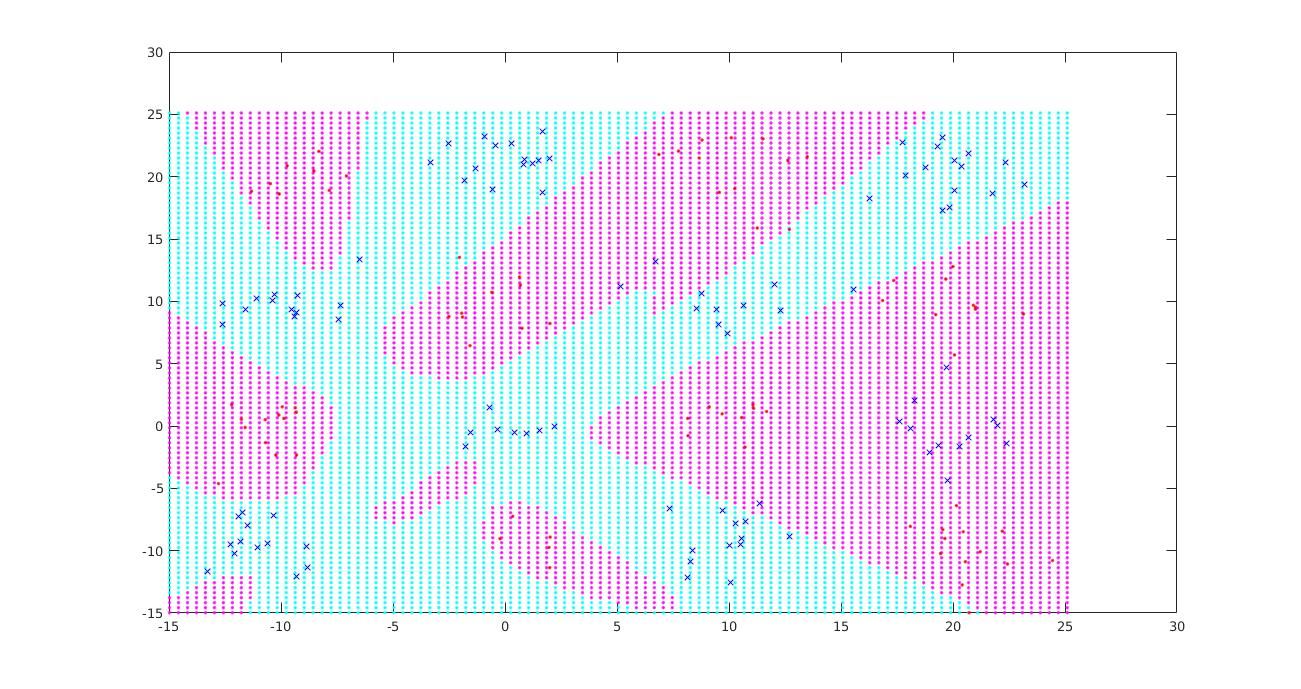
\includegraphics[scale=.3]{figures/exercise_02_08_02_fig_58.jpg}
        \caption{No.Hidden Layers = 10}
    \end{subfigure}\\
    \begin{subfigure}[h]{0.5\textwidth}
        \centering
        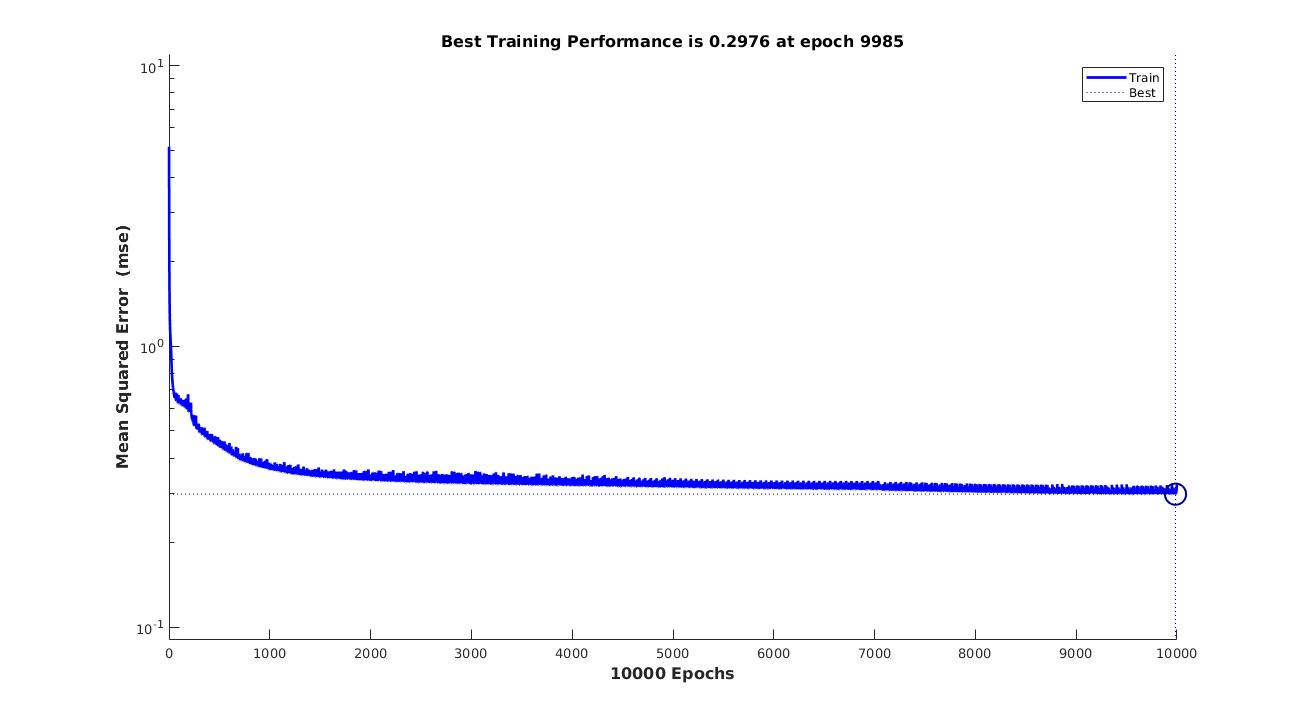
\includegraphics[scale=.3]{figures/exercise_02_08_02_fig_59.jpg}
        \caption{No.Hidden Layers = 10}
    \end{subfigure}\\
\end{figure}

\newpage

\begin{figure}[ht]
    \begin{subfigure}[h]{0.5\textwidth}
        \centering
        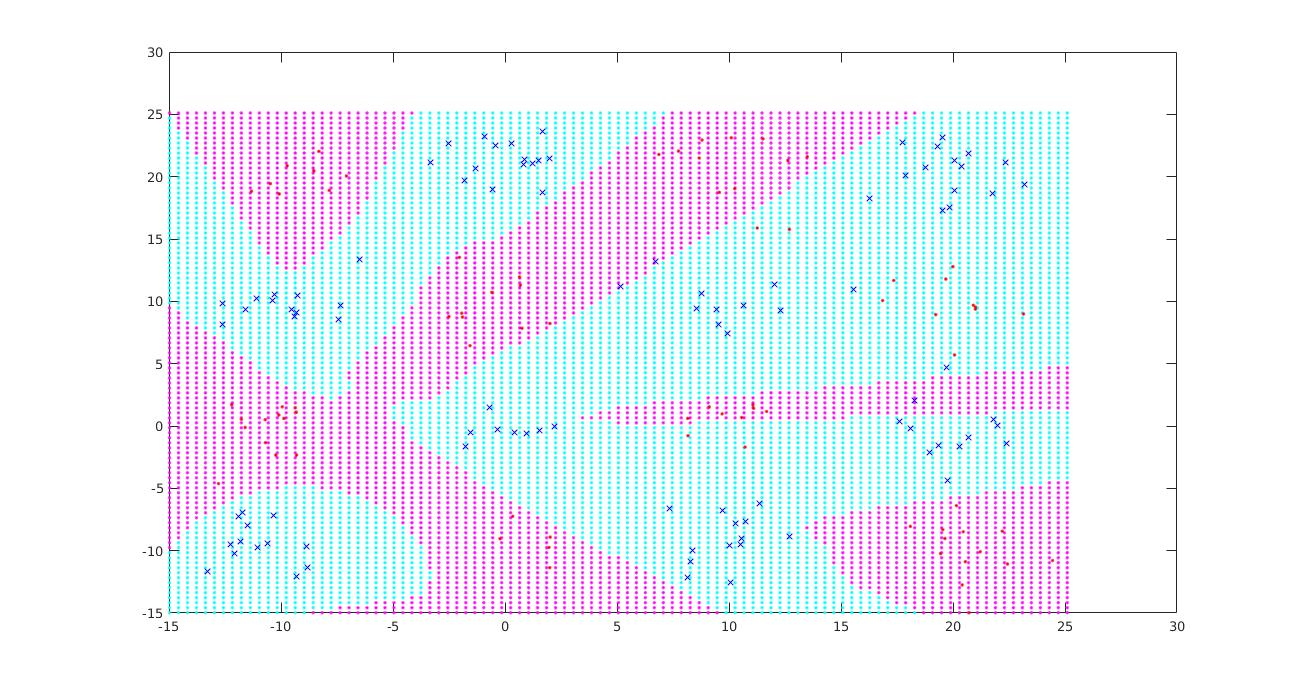
\includegraphics[scale=.3]{figures/exercise_02_08_02_fig_61.jpg}
        \caption{No.Hidden Layers = 14}
    \end{subfigure}\\
    \begin{subfigure}[h]{0.5\textwidth}
        \centering
        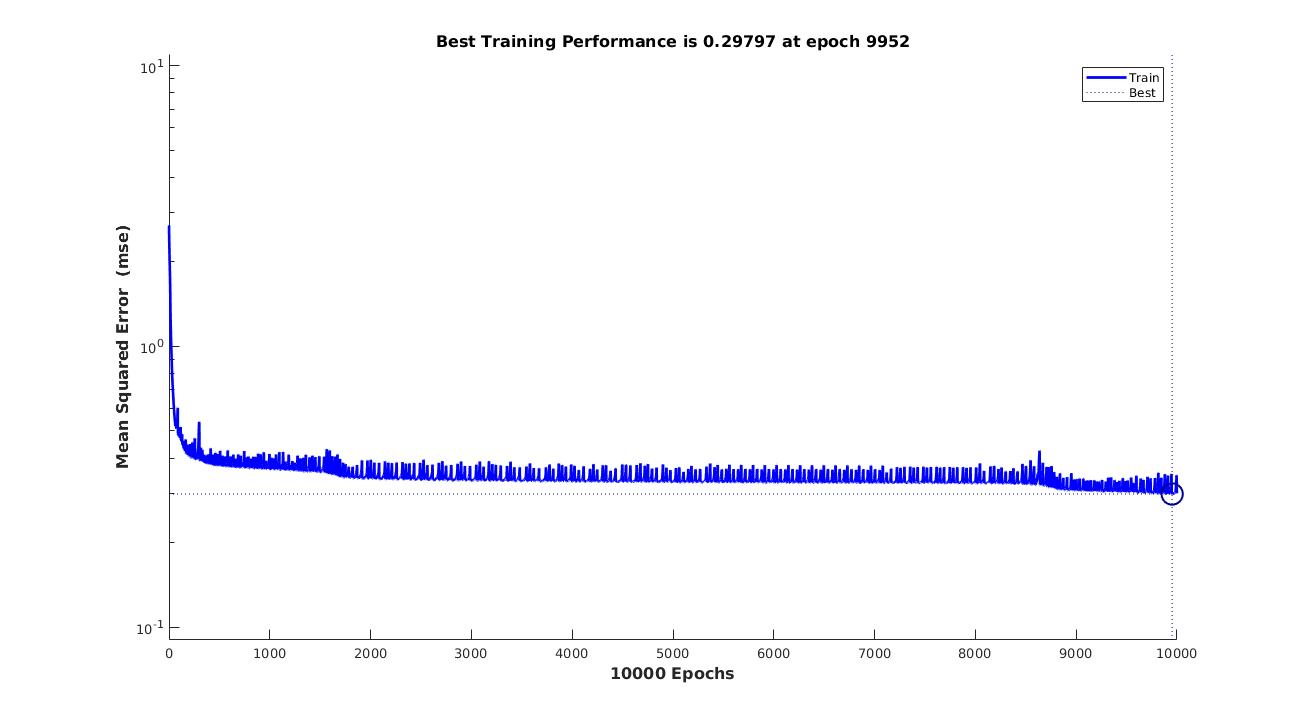
\includegraphics[scale=.3]{figures/exercise_02_08_02_fig_62.jpg}
        \caption{No.Hidden Layers = 14}
    \end{subfigure}\\
\end{figure}

\newpage

\begin{figure}[ht]
    \begin{subfigure}[h]{0.5\textwidth}
        \centering
        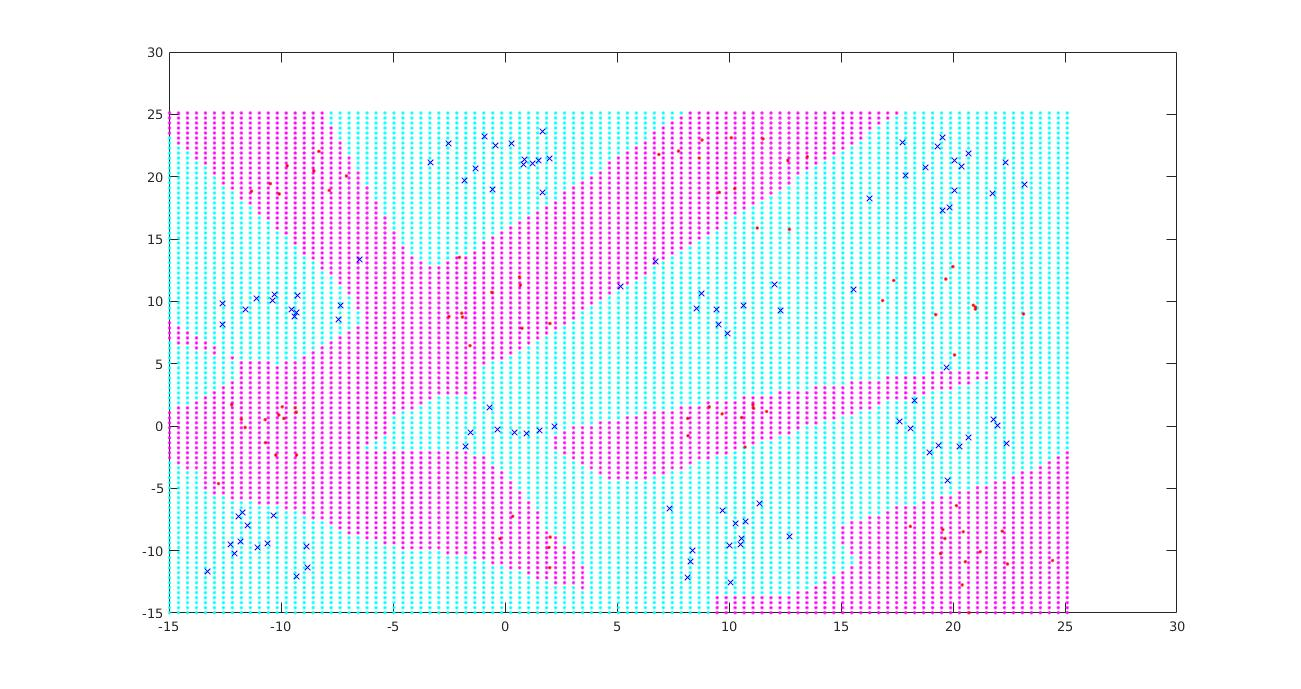
\includegraphics[scale=.3]{figures/exercise_02_08_02_fig_64.jpg}
        \caption{No.Hidden Layers = 16}
    \end{subfigure}\\
    \begin{subfigure}[h]{0.5\textwidth}
        \centering
        \includegraphics[scale=.3]{figures/exercise_02_08_02_fig_65.jpg}
        \caption{No.Hidden Layers = 16}
    \end{subfigure}\\
\end{figure}

\newpage

\begin{figure}[ht]
    \begin{subfigure}[h]{0.5\textwidth}
        \centering
        \includegraphics[scale=.3]{figures/exercise_02_08_02_fig_67.jpg}
        \caption{No.Hidden Layers = 20}
    \end{subfigure}\\
    \begin{subfigure}[h]{0.5\textwidth}
        \centering
        \includegraphics[scale=.3]{figures/exercise_02_08_02_fig_68.jpg}
        \caption{No.Hidden Layers = 20}
    \end{subfigure}\\
\end{figure}

\newpage

\begin{figure}[ht]
    \begin{subfigure}[h]{0.5\textwidth}
        \centering
        \includegraphics[scale=.3]{figures/exercise_02_08_02_fig_70.jpg}
        \caption{No.Hidden Layers = 32}
    \end{subfigure}\\
    \begin{subfigure}[h]{0.5\textwidth}
        \centering
        \includegraphics[scale=.3]{figures/exercise_02_08_02_fig_71.jpg}
        \caption{No.Hidden Layers = 32}
    \end{subfigure}\\
\end{figure}

\newpage

\begin{figure}[ht]
    \begin{subfigure}[h]{0.5\textwidth}
        \centering
        \includegraphics[scale=.3]{figures/exercise_02_08_02_fig_73.jpg}
        \caption{No.Hidden Layers = 40}
    \end{subfigure}\\
    \begin{subfigure}[h]{0.5\textwidth}
        \centering
        \includegraphics[scale=.3]{figures/exercise_02_08_02_fig_74.jpg}
        \caption{No.Hidden Layers = 40}
    \end{subfigure}\\
\end{figure}

\newpage

\begin{figure}[ht]
    \centering
    \includegraphics[scale=.4]{figures/exercise_02_08_02_fig_77.jpg}
    \caption{Training and Test Error with $\sigma=3$}
\end{figure}

\newpage
\subsubsection{$\sigma=4$}

\begin{center}
\begin{tabular}{ |p{3.5cm}|p{1.2cm}|p{1.2cm}| }
\hline
\multicolumn{3}{|c|}{Test and Training Errors with $\sigma=4$} \\
\hline
No.Hidden Layers & Training & Test \\
\hline
7 & 0.1444 & 0.1611\\
8 & 0.1500 & 0.2000\\
10 & 0.1111 & 0.2111\\
14 & 0.1167 & 0.2389\\
16 & 0.1389 & 0.1833\\
20 & 0.0500 & 0.1444\\
32 & 0.0333 & 0.1389\\
40 & 0.0278 & 0.1500\\
\hline
\end{tabular}
\end{center}

\newpage
\begin{figure}[ht]
        \centering
        \includegraphics[scale=0.3]{figures/exercise_02_08_02_fig_01.jpg}
        \caption{Training Data X1 with $\sigma=4$}
\end{figure}

\newpage

\begin{figure}[ht]
    \begin{subfigure}[h]{0.5\textwidth}
        \centering
        \includegraphics[scale=.3]{figures/exercise_02_08_02_fig_04.jpg}
        \caption{No.Hidden Layers = 7}
    \end{subfigure}\\
    \begin{subfigure}[ht]{0.5\textwidth}
        \centering
        \includegraphics[scale=.3]{figures/exercise_02_08_02_fig_02.jpg}
        \caption{No.Hidden Layers = 7}
    \end{subfigure}\\
\end{figure}

\newpage

\begin{figure}[ht]
    \begin{subfigure}[h]{0.5\textwidth}
        \centering
        \includegraphics[scale=.3]{figures/exercise_02_08_02_fig_05.jpg}
        \caption{No.Hidden Layers = 8}
    \end{subfigure}\\
    \begin{subfigure}[h]{0.5\textwidth}
        \centering
        \includegraphics[scale=.3]{figures/exercise_02_08_02_fig_06.jpg}
        \caption{No.Hidden Layers = 8}
    \end{subfigure}\\
\end{figure}

\newpage

\begin{figure}[ht]
    \begin{subfigure}[h]{0.5\textwidth}
        \centering
        \includegraphics[scale=.3]{figures/exercise_02_08_02_fig_08.jpg}
        \caption{No.Hidden Layers = 10}
    \end{subfigure}\\
    \begin{subfigure}[h]{0.5\textwidth}
        \centering
        \includegraphics[scale=.3]{figures/exercise_02_08_02_fig_09.jpg}
        \caption{No.Hidden Layers = 10}
    \end{subfigure}\\
\end{figure}

\newpage

\begin{figure}[ht]
    \begin{subfigure}[h]{0.5\textwidth}
        \centering
        \includegraphics[scale=.3]{figures/exercise_02_08_02_fig_11.jpg}
        \caption{No.Hidden Layers = 14}
    \end{subfigure}\\
    \begin{subfigure}[h]{0.5\textwidth}
        \centering
        \includegraphics[scale=.3]{figures/exercise_02_08_02_fig_12.jpg}
        \caption{No.Hidden Layers = 14}
    \end{subfigure}\\
\end{figure}

\newpage

\begin{figure}[ht]
    \begin{subfigure}[h]{0.5\textwidth}
        \centering
        \includegraphics[scale=.3]{figures/exercise_02_08_02_fig_14.jpg}
        \caption{No.Hidden Layers = 16}
    \end{subfigure}\\
    \begin{subfigure}[h]{0.5\textwidth}
        \centering
        \includegraphics[scale=.3]{figures/exercise_02_08_02_fig_15.jpg}
        \caption{No.Hidden Layers = 16}
    \end{subfigure}\\
\end{figure}

\newpage

\begin{figure}[ht]
    \begin{subfigure}[h]{0.5\textwidth}
        \centering
        \includegraphics[scale=.3]{figures/exercise_02_08_02_fig_17.jpg}
        \caption{No.Hidden Layers = 20}
    \end{subfigure}\\
    \begin{subfigure}[h]{0.5\textwidth}
        \centering
        \includegraphics[scale=.3]{figures/exercise_02_08_02_fig_18.jpg}
        \caption{No.Hidden Layers = 20}
    \end{subfigure}\\
\end{figure}

\newpage

\begin{figure}[ht]
    \begin{subfigure}[h]{0.5\textwidth}
        \centering
        \includegraphics[scale=.3]{figures/exercise_02_08_02_fig_20.jpg}
        \caption{No.Hidden Layers = 32}
    \end{subfigure}\\
    \begin{subfigure}[h]{0.5\textwidth}
        \centering
        \includegraphics[scale=.3]{figures/exercise_02_08_02_fig_22.jpg}
        \caption{No.Hidden Layers = 32}
    \end{subfigure}\\
\end{figure}

\newpage

\begin{figure}[ht]
    \begin{subfigure}[h]{0.5\textwidth}
        \centering
        \includegraphics[scale=.3]{figures/exercise_02_08_02_fig_23.jpg}
        \caption{No.Hidden Layers = 40}
    \end{subfigure}\\
    \begin{subfigure}[h]{0.5\textwidth}
        \centering
        \includegraphics[scale=.3]{figures/exercise_02_08_02_fig_24.jpg}
        \caption{No.Hidden Layers = 40}
    \end{subfigure}\\
\end{figure}

\begin{figure}[ht]
    \centering
    \includegraphics[scale=.4]{figures/exercise_02_08_02_fig_78.jpg}
    \caption{Training and Test Error with $\sigma=4$}
\end{figure}

\end{homeworkProblem}

%----------------------------------------------------------------------------------------
\end{document}
